\documentclass[runningheads]{llncs}

% Basic packages
\usepackage{amsmath,amssymb}
\usepackage{tikz}
\usetikzlibrary{arrows.meta,positioning,shapes,graphs,calc}
\usepackage{pgfplots}
\pgfplotsset{compat=1.17}
\usepackage{xcolor}
\usepackage{array}
\usepackage{tabularx}
\usepackage{hyperref}
\usepackage{microtype}
\usepackage{float}

% Unicode font support (required for Agda output - compile with lualatex)
\usepackage{fontspec}
\usepackage{unicode-math}

\setmainfont{DejaVu Serif}
\setsansfont{DejaVu Sans}
\setmonofont{DejaVu Sans Mono}[Scale=MatchLowercase]
\setmathfont{STIX Two Math}

% Agda literate support
\usepackage{agda}
\usepackage{agda-spec}

\renewcommand{\AgdaFontStyle}[1]{{\small\sffamily #1}}
\renewcommand{\AgdaKeywordFontStyle}[1]{{\small\sffamily\bfseries #1}}
\renewcommand{\AgdaBoundFontStyle}[1]{{\small\sffamily\itshape #1}}
\renewcommand{\AgdaStringFontStyle}[1]{{\small\ttfamily #1}}
\renewcommand{\AgdaCommentFontStyle}[1]{{\small\ttfamily #1}}

% Nord-inspired Agda colors
\definecolor{AgdaComment}      {HTML}{616E88}
\definecolor{AgdaPragma}       {HTML}{616E88}
\definecolor{AgdaKeyword}      {HTML}{5E81AC}
\definecolor{AgdaString}       {HTML}{A3BE8C}
\definecolor{AgdaNumber}       {HTML}{B48EAD}
\definecolor{AgdaSymbol}       {HTML}{4C566A}

\definecolor{AgdaBound}                 {HTML}{2E3440}
\definecolor{AgdaGeneralizable}         {HTML}{5E81AC}
\definecolor{AgdaInductiveConstructor}  {HTML}{8FBCBB}
\definecolor{AgdaCoinductiveConstructor}{HTML}{88C0D0}
\definecolor{AgdaDatatype}              {HTML}{81A1C1}
\definecolor{AgdaField}                 {HTML}{B48EAD}
\definecolor{AgdaFunction}              {HTML}{5E81AC}
\definecolor{AgdaMacro}                 {HTML}{A3BE8C}
\definecolor{AgdaModule}                {HTML}{E0BA62}
\definecolor{AgdaPostulate}             {HTML}{BF616A}
\definecolor{AgdaPrimitive}             {HTML}{81A1C1}
\definecolor{AgdaRecord}                {HTML}{81A1C1}
\definecolor{AgdaArgument}              {HTML}{4C566A}

\definecolor{nord0}{HTML}{2E3440}
\definecolor{nord1}{HTML}{3B4252}
\definecolor{nord2}{HTML}{434C5E}
\definecolor{nord3}{HTML}{4C566A}
\definecolor{nord4}{HTML}{D8DEE9}
\definecolor{nord5}{HTML}{E5E9F0}
\definecolor{nord6}{HTML}{ECEFF4}
\definecolor{nord7}{HTML}{8FBCBB}
\definecolor{nord8}{HTML}{88C0D0}
\definecolor{nord9}{HTML}{81A1C1}
\definecolor{nord10}{HTML}{5E81AC}
\definecolor{nord11}{HTML}{BF616A}
\definecolor{nord12}{HTML}{D08770}
\definecolor{nord13}{HTML}{EBCB8B}
\definecolor{nord14}{HTML}{A3BE8C}
\definecolor{nord15}{HTML}{B48EAD}

\urlstyle{tt}
\newcommand{\fpath}[1]{\nolinkurl{#1}}

% Theorem environments (theorem, lemma, corollary, definition, remark)
% are predefined by the llncs class.

\title{Coinductive Symmetric Homomorphism Reinforcement Learning:\\
Optimality as Structure Preservation}
\titlerunning{Coinductive Symmetric Homomorphism RL}

\author{Anonymous Author(s)}
\authorrunning{Anonymous Author(s)}
\institute{Anonymous Institution}

\begin{document}

\maketitle

\begin{abstract}
We define a typable optimality criterion based on coinductive preservation of action dominance: an action is better than another if it leads to a strictly better future in the coinductive sense.
We realize this criterion through homomorphic rankings---permutations of the action set that preserve the coinductive ordering on successor value streams.

A natural strengthening additionally requires immediate rewards to respect the ranking.
These two conditions decompose cleanly; the homomorphism criterion alone is strictly more general and correctly ranks actions in sacrifice patterns where discounted return fails.
We give a constructive procedure---the Finder together with violation-correction learning---that computes rankings provably satisfying the criterion.
All results are machine-verified in Agda, including monotonic convergence of learning, instant adaptation, stochastic lifting via the Giry monad, and scalable verification on large combinatorial domains with zero postulates.

\keywords{Reinforcement learning \and Coinduction \and Symmetric group \and Formal verification \and Agda \and Optimality \and Stochastic dominance}
\end{abstract}

\noindent\textbf{Code Availability.}
All definitions, theorems, and algorithms presented in this paper have been formalized and machine-checked in Agda 2.8.0.
The complete development includes the \texttt{CoinductiveHomomorphism} and \texttt{CoindHomo} records, the Finder algorithm, monotonic convergence of learning, instant adaptation, stochastic lifting via the finite distribution monad, the Environment Class infrastructure, compositional algebra, verified state abstraction, and all verified tasks (including \texttt{Queens8}).
Concrete module paths are referenced throughout the text; the full artifact will be made publicly available upon acceptance.

%%%%%%%%%%%%%%%%%%%%%%%%%%%%%%%%%%%%%%%%%%%%%%%%%%%%%%%%%%%%%%%%%%%%%%%%%%%%%%%
% PART I: MOTIVATION
%%%%%%%%%%%%%%%%%%%%%%%%%%%%%%%%%%%%%%%%%%%%%%%%%%%%%%%%%%%%%%%%%%%%%%%%%%%%%%%

\section{Motivation: The Limitations of Scalar Returns}

Reinforcement learning (RL) studies agents that learn to make sequential decisions by interacting with an environment~\cite{Sutton2018}.  At each discrete time step, the agent observes a \emph{state}, selects an \emph{action}, and receives a numerical \emph{reward} that signals how good the outcome was.  The agent's goal is to find a \emph{policy}---a rule mapping states to actions---that collects as much reward as possible over time.

The question is how to define ``as much reward as possible.''  The dominant answer in modern RL is the \emph{expected discounted return}: given a policy~$\pi$, the agent averages over all trajectories~$\tau$ it might experience:
\[
J(\pi) = \mathbb{E}_{\tau \sim \pi} \left[ \sum_{t=0}^{\infty} \gamma^t r_t \right]
\]
where $r_t$ is the reward at time~$t$ and $\gamma \in [0,1)$ is the \emph{discount factor}.  The discount makes future rewards exponentially less valuable: a reward 10~steps ahead counts for only~$\gamma^{10}$ of its face value.  This ensures the sum converges and makes the problem mathematically tractable.

The result is a single scalar.  A policy is optimal when it maximizes this number.  This formulation---rooted in Bellman's dynamic programming principle \cite{Bellman1957} and operationalized by algorithms like Q-learning \cite{Watkins1992}, policy gradient methods, and deep RL \cite{Mnih2015}---has driven remarkable successes, from game playing to robotics.

\subsection{The Problem: Temporal Structure Loss}

Scalar return collapses the temporal structure of reward sequences.  Two futures can have similar discounted sums while being structurally very different:

\begin{center}
\begin{tabular}{lcc}
\textbf{Future} & \textbf{Reward Sequence} & \textbf{Sum ($\gamma{=}0.9$)} \\
\hline
A: ``Win then die'' & $[10, -5, 0, 0, \ldots]$ & $10 - 4.5 = 5.5$ \\
B: ``Struggle then thrive'' & $[0, 5, 0, 0, \ldots]$ & $0 + 4.5 = 4.5$ \\
\end{tabular}
\end{center}

A scalar optimizer prefers A, yet B is structurally superior---it avoids catastrophic failure and reaches a productive state.  This is \textbf{value aliasing}: structurally different futures map to the same scalar.

This formulation introduces several artifacts:
\begin{itemize}
\item \textbf{Discount factor ($\gamma$):} An extrinsic parameter that undervalues delayed rewards and can make the optimal policy discontinuous in $\gamma$.
\item \textbf{Instability:} Q-learning's bootstrapping of scalar estimates leads to the deadly triad (function approximation $+$ bootstrapping $+$ off-policy learning) \cite{Sutton2018}.
\item \textbf{Credit assignment:} Rewards at large $t$ are effectively zero under discounting, crippling long-horizon learning.
\end{itemize}

\noindent These are not bugs---they follow directly from compressing sequences into scalars.  When optimal behavior requires paying a cost now for a benefit later, discounting systematically distorts the decision.

\subsection{Our Approach}

We instead define optimality via \emph{structure preservation}.  We keep reward sequences as infinite streams and rank actions by whether they lead to successor states whose optimal futures dominate others at every depth under a coinductive ordering.  The central question is what structure to preserve and how to do so formally.

%%%%%%%%%%%%%%%%%%%%%%%%%%%%%%%%%%%%%%%%%%%%%%%%%%%%%%%%%%%%%%%%%%%%%%%%%%%%%%%
% PART II: THE IDEA
%%%%%%%%%%%%%%%%%%%%%%%%%%%%%%%%%%%%%%%%%%%%%%%%%%%%%%%%%%%%%%%%%%%%%%%%%%%%%%%

\section{Structural Optimality: Successor State Quality}\label{sec:key-idea}

Consider an agent choosing between two actions at a state.  Action~$a$ gives an immediate reward of~$3$ but leads to a dead-end state (reward~$0$ forever).  Action~$b$ gives immediate reward~$0$ but leads to a productive state (reward~$5$ forever).

A scalar return optimizer with low discount factor might prefer~$a$.  But structurally, $b$ is the better action---it leads to a \emph{better state}.  The immediate reward is a one-time cost; the successor state quality compounds forever.

This motivates our central criterion:

\begin{quote}
\textbf{An action is ranked higher because it leads to a successor state of higher quality.}  A state is of higher quality when acting optimally from it yields higher rewards at every future depth---which itself depends on the quality of states reachable from there, unfolding coinductively.
\end{quote}

The ranking tracks which actions lead to \emph{success}---both in the sense of successor state and in the evaluative sense.

%%%%%%%%%%%%%%%%%%%%%%%%%%%%%%%%%%%%%%%%%%%%%%%%%%%%%%%%%%%%%%%%%%%%%%%%%%%%%%%
% PART III: FORMAL DEFINITION
%%%%%%%%%%%%%%%%%%%%%%%%%%%%%%%%%%%%%%%%%%%%%%%%%%%%%%%%%%%%%%%%%%%%%%%%%%%%%%%

\section{Formal Definition}\label{sec:formal}

\subsection{The Order Homomorphism}

We now make the intuition from Section~\ref{sec:key-idea} precise.  The formalization requires three ingredients; we introduce each in turn.

\paragraph{Actions and rankings.}
Let $\mathcal{A}$ be the finite set of actions available to the agent.
At each state~$s$, the agent maintains a \emph{ranking}---a total preorder $\le_a$ on~$\mathcal{A}$---expressing which actions it considers at least as good as which others.
If $a \le_a b$, the agent regards~$b$ as at least as good as~$a$ at state~$s$.

The object of interest is the \emph{entire} order on~$\mathcal{A}$, not merely its maximum.  A total preorder commits the agent to comparing \emph{every} pair of actions---including the two \emph{worst} ones---rather than only separating a top choice from the rest.  A strict total ranking is precisely an element of the symmetric group~$S_{|\mathcal{A}|}$ acting on the actions: the agent selects one ordering among all~$|\mathcal{A}|!$ permutations, whereas an argmax commitment leaves that choice almost entirely underdetermined.  This full-ranking stance is foundational---it is the sense in which the homomorphism is \emph{symmetric}: optimality is judged against the whole permutation structure on actions, not a single distinguished action.  An agent that has genuinely understood an environment can say which of even its two worst options is less bad; an argmax-centric agent cannot.  The commitment is not merely conceptual: it is what makes learning correct \emph{every} violated pair, including among the worst (\S\ref{sec:learning}), and what makes adaptation to a lost top action an $O(1)$ lookup of the next-best (\S\ref{sec:adaptation}).

\paragraph{Successor states.}
When the agent takes action~$a$ at state~$s$, the environment transitions to a new state and emits a reward.
We write $\mathit{step}(s,a)$ for this transition, which produces a pair: the successor state~$\mathit{next}(s,a)$ and the immediate reward~$r(s,a)$.
The successor state is where the agent \emph{ends up}---the starting point of the rest of its life.

\paragraph{Value streams.}
From any state~$s'$, the agent can act optimally into the indefinite future, collecting a reward at each time step.
Rather than collapsing this sequence into a scalar, we keep it as an infinite stream:
\[
\mathit{value}(s') = \bigl[\, v_0,\; v_1,\; v_2,\; \ldots \,\bigr]
\]
where $v_t$ is the optimal reward achievable at depth~$t$ from~$s'$.
This stream retains the full temporal structure that a scalar return discards.
(The precise construction is given in \S\ref{sec:agda-core}.)

\paragraph{Comparing streams.}
To say one state is ``better'' than another, we compare their value streams \emph{pointwise}.
We write $x \le_s y$ when stream~$x$ is dominated by stream~$y$ at every position: for all $t = 0, 1, 2, \ldots$, the $t$-th element of~$x$ is~$\le_r$ the $t$-th element of~$y$.
This is a strong condition: the better stream must be at least as good at every single future depth, not just on average or in total.

\medskip

With these ingredients in hand, the definition is a single sentence:

\begin{definition}[CoinductiveHomomorphism --- Successor Condition]\label{def:coind-homo}
The ranking $\le_a$ satisfies the \textbf{CoinductiveHomomorphism} condition at state~$s$ if:
\[
a \le_a b \;\;\Longrightarrow\;\; \mathit{value}(\mathit{next}(s,a)) \le_s \mathit{value}(\mathit{next}(s,b))
\]
\end{definition}

\noindent In words: if the ranking says~$b$ is at least as good as~$a$, then the state reached by~$b$ must have a value stream that dominates the value stream of the state reached by~$a$---at every future depth, without exception.

The definition says nothing about the immediate rewards $r(s,a)$ and $r(s,b)$.
It judges actions entirely by \emph{where they lead}.
An action that pays a cost now but reaches a superior state is correctly ranked, because the successor state's value stream---reflecting the entire optimal future from that point onward---is what matters.

\paragraph{Why ``homomorphism''?}
The map $a \mapsto \mathit{value}(\mathit{next}(s,a))$ sends each action to a stream.
The definition requires this map to be \emph{order-preserving}: if $a \le_a b$ in the action ranking, then $\mathit{value}(\mathit{next}(s,a)) \le_s \mathit{value}(\mathit{next}(s,b))$ in the stream ordering.
An order-preserving map between ordered sets is called a \emph{homomorphism}---it preserves the structure.
The qualifier ``coinductive'' refers to the target: the stream ordering $\le_s$ unfolds to arbitrary depth, verified one position at a time, without bound---an infinite tower of commuting diagrams:

\begin{figure}[H]
\centering
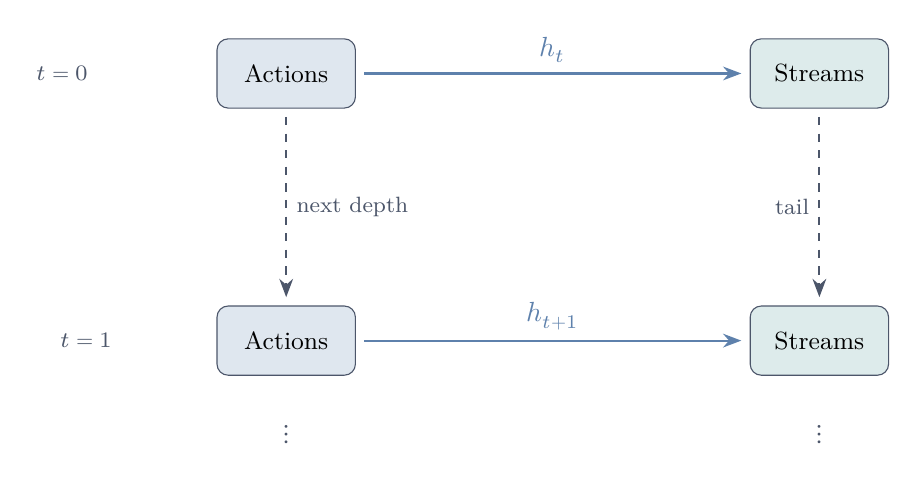
\begin{tikzpicture}[
    node distance=2.5cm and 5cm,
    obj/.style={draw=nord3,rounded corners,minimum height=2.5em,minimum width=5em,align=center,font=\small,fill=nord5},
    arr/.style={->,thick,>=Stealth,shorten >=3pt,shorten <=3pt,nord10}
]
\node[obj,fill=nord9!25] (A1) {Actions};
\node[obj,fill=nord7!30,right=of A1] (S1) {Streams};
\draw[arr] (A1) -- node[above,color=nord10] {$h_t$} (S1);

\node[obj,fill=nord9!25,below=of A1] (A2) {Actions};
\node[obj,fill=nord7!30,right=of A2] (S2) {Streams};
\draw[arr] (A2) -- node[above,color=nord10] {$h_{t+1}$} (S2);

\draw[arr,dashed,nord3] (A1) -- node[right,font=\footnotesize,color=nord3] {next depth} (A2);
\draw[arr,dashed,nord3] (S1) -- node[left,font=\footnotesize,color=nord3] {tail} (S2);

\node[below=0.5cm of A2,color=nord3] {$\vdots$};
\node[below=0.5cm of S2,color=nord3] {$\vdots$};

\node[left=1.5cm of A1,font=\footnotesize,color=nord3] {$t=0$};
\node[left=1.2cm of A2,font=\footnotesize,color=nord3] {$t=1$};
\end{tikzpicture}
\caption{The coinductive tower: $h_t$ maps each action to its successor-value stream at depth~$t$.  Ranking preservation ($a \le_a b \Rightarrow h_t(a) \le_s h_t(b)$) must hold at every level, verified by unfolding one \texttt{tail} at a time.}
\label{fig:tower}
\end{figure}

This is a \textbf{strategic} evaluation of actions: it assesses the absolute potential of the successor state, allowing for immediate tactical sacrifices.

\subsection{The Action-Value Specialization}

The CoinductiveHomomorphism condition evaluates successor state quality---the agent's future \emph{after} the transition.  A natural strengthening evaluates the \emph{entire} consequence of an action, including the immediate reward it produces.

Given action~$a$ at state~$s$, define the \emph{action-value stream}:
\[
\mathit{action\text{-}value}(s,a) = \bigl[\, r(s,a),\;\; v_0,\;\; v_1,\;\; v_2,\;\; \ldots \,\bigr]
\]
Its head is the immediate transition reward; its tail is the value stream of the successor state.  The action-value stream is a richer object: it records both what the action pays now and what it sets up for the future.

\begin{definition}[CoindHomo --- Action-Value Condition]\label{def:coindhomo}
The ranking $\le_a$ satisfies the \textbf{CoindHomo} (action-value) condition at state~$s$ if:
\[
a \le_a b \;\;\Longrightarrow\;\; \mathit{action\text{-}value}(s,a) \le_s \mathit{action\text{-}value}(s,b)
\]
\end{definition}

\noindent Because $\le_s$ compares streams pointwise, this bundles \emph{two} requirements into one: the immediate rewards must compare correctly (the head), \emph{and} the successor state qualities must compare correctly (the tail).

This is a \textbf{tactical} evaluation: it demands that the better-ranked action wins both the immediate payoff and the long-term future.  When both conditions hold, the ranking is unassailable.  But when the optimal action sacrifices immediate reward for a superior successor---the pattern from Section~\ref{sec:key-idea}---the head condition breaks, and this definition cannot express the correct ranking.

\subsection{Decomposition}

The relationship between the two definitions is precise:

\begin{theorem}[Decomposition]\label{thm:decomposition}
The action-value condition decomposes into two independent conditions:
\begin{enumerate}
\item \textbf{Successor quality} (CoinductiveHomomorphism): $a \le_a b \implies \mathit{value}(\mathit{next}(s,a)) \le_s \mathit{value}(\mathit{next}(s,b))$
\item \textbf{Immediate reward compatibility}: $a \le_a b \implies r(s,a) \le_r r(s,b)$
\end{enumerate}
Either condition can hold independently.  Together, they are equivalent to the action-value condition.
\end{theorem}

The first condition is CoinductiveHomomorphism---the strategic evaluation.
The second is a purely local constraint on immediate rewards.
The action-value condition is their conjunction: it insists on tactical \emph{and} strategic soundness simultaneously.

When immediate rewards are aligned with the ranking---as they are in environments with uniform step costs, shaped rewards, or goal-terminal structure---the second condition holds for free, and the two definitions coincide.  The gap opens only in environments where the optimal action has a worse immediate reward than a suboptimal alternative: the sacrifice pattern.

As sets of admissible rankings the relationship is a strict containment, $\mathrm{CoindHomo} \subsetneq \mathrm{CoinductiveHomomorphism}$: uniform-step-cost environments lie in the inner set, while sacrifice-now-gain-later environments lie in the gap.

%%%%%%%%%%%%%%%%%%%%%%%%%%%%%%%%%%%%%%%%%%%%%%%%%%%%%%%%%%%%%%%%%%%%%%%%%%%%%%%
% PART IV: THE AGDA CORE
%%%%%%%%%%%%%%%%%%%%%%%%%%%%%%%%%%%%%%%%%%%%%%%%%%%%%%%%%%%%%%%%%%%%%%%%%%%%%%%

\section{The Agda Core}\label{sec:agda-core}

We now present the verified implementation.  Every code listing shown below is type-checked by Agda; the snippets are rendered directly from the checked source.

\begin{code}[hide]
{-# OPTIONS --safe --guardedness #-}

module paper where

open import Data.List using (List; map; foldr; []; _∷_)
open import Codata.Guarded.Stream using (Stream; head; tail; _∷_; tabulate)
open import Relation.Binary.PropositionalEquality using (_≡_; _≢_; refl)
open import Data.Product using (proj₁; proj₂; _×_; _,_)
open import Relation.Nullary using (¬_; Dec; yes; no)
open import Function using (_∘_)
open import Data.Nat using (ℕ; zero; suc; _⊔_)
open import Data.Bool using (Bool; true; false; if_then_else_)
\end{code}

The \texttt{Core} module is parameterized by the environment:

\begin{code}[hide]
module Core
  (State Action Reward : Set)
  (step                : State → Action → State × Reward)
  (_≤ᵣ_                : Reward → Reward → Set)
  (max                 : Reward → Reward → Reward)
  (bottom              : Reward)
  (all-actions         : List Action)
  where

  infix 4 _≤ₛ_

  StreamR : Set
  StreamR = Stream Reward

  max-list : List Reward → Reward
  max-list = foldr max bottom
\end{code}

\subsection{Value and Action-Value Streams}

The key construction: \texttt{value} is an infinite stream obtained by tabulating finite-horizon solutions.

\begin{code}
  solve : State → ℕ → Reward
  solve s zero    = max-list (map (λ a → proj₂ (step s a)) all-actions)
  solve s (suc n) = max-list (map (λ a → solve (proj₁ (step s a)) n) all-actions)

  value : State → StreamR
  value s = tabulate (solve s)

  action-value : State → Action → StreamR
  head (action-value s a) = proj₂ (step s a)
  tail (action-value s a) = value (proj₁ (step s a))
\end{code}

\noindent \texttt{solve~s~n} computes the maximum reward achievable \emph{exactly~$n$ steps from now}, independently maximizing the action at every intermediate step.  Crucially, the action sequence that maximizes the reward at depth~$n$ may differ from the one that maximizes at depth~$m$.  The resulting value stream is therefore \emph{not a trajectory}---no single action sequence produces it.  It is the pointwise upper envelope of all possible trajectories: the agent's \textbf{capability profile} from state~$s$, recording the best it \emph{could} achieve at each future depth.

CoinductiveHomomorphism compares these capability profiles.  When state~$s_b$'s profile dominates~$s_a$'s at every depth, the agent prefers any action that reaches~$s_b$---even if that action sacrifices immediate reward.  The sacrifice is invisible in the profile: it only records what the agent \emph{can} reach, not the cost of getting there.

The \texttt{action-value} of action~$a$ at state~$s$ is a stream whose head is the immediate reward and whose tail is the capability profile of the successor state.

\subsection{Coinductive Stream Ordering}

\begin{code}
  record _≤ₛ_ (x y : StreamR) : Set where
    coinductive
    field
      head≤ : head x ≤ᵣ head y
      tail≤ : tail x ≤ₛ tail y

  open _≤ₛ_ public
\end{code}

\noindent A proof of $x \le_s y$ is an infinite witness: at every time step, the heads compare correctly.

\subsection{Why Propositions Instead of Booleans?}\label{sec:props-vs-bools}

The reward ordering \texttt{\_$\le$ᵣ\_} lives in \texttt{Set}---it is a \emph{proposition}, not a Boolean decision procedure.  This is a deliberate design choice:

\begin{itemize}
\item \textbf{Booleans are blind:} \texttt{true} carries no information about \emph{why} the comparison holds.  To use a Boolean result in a proof, a separate soundness lemma is required.
\item \textbf{Propositions carry evidence:} A value of type \texttt{r₁ $\le$ᵣ r₂} \emph{is} the proof---no lemma needed.
\item \textbf{Decidability bridges both:} \texttt{Dec (r₁ $\le$ᵣ r₂)} is either \texttt{yes p} (with proof~\texttt{p}) or \texttt{no ¬p} (with refutation).
\end{itemize}

\noindent This separation threads through the entire architecture: the Core module uses propositions for proofs; the Finder uses Booleans for speed; the Environment Class infrastructure bridges them via \texttt{Dec}.

\subsection{CoindHomo: The Action-Value Condition}

The \texttt{CoindHomo} record is the Agda encoding of the Action-Value Coinductive Homomorphism (Definition~\ref{def:coindhomo}):

\begin{code}
  record CoindHomo : Set₁ where
    field
      _≤ₐ_      : State → Action → Action → Set
      preserves : ∀ a b s → _≤ₐ_ s a b →
                  action-value s a ≤ₛ action-value s b

  open CoindHomo {{...}} public
\end{code}

\noindent The record has two fields.  The first, \texttt{\_$\le$ₐ\_}, is the ranking itself---a ternary relation indexed by state, taking two actions and returning a type (a proposition, per \S\ref{sec:props-vs-bools}).  The second, \texttt{preserves}, is the proof obligation: for any actions~$a, b$ and state~$s$, if the ranking says $a \le_a b$, then the full action-value stream of~$a$ is coinductively dominated by that of~$b$.  Because $\le_s$ checks both head and tail, this bundles two requirements: the immediate reward must compare correctly (head), and the successor state quality must compare correctly (tail).

\subsection{CoinductiveHomomorphism: The Successor Condition}

The \texttt{CoinductiveHomomorphism} record is the Agda encoding of Definition~\ref{def:coind-homo}.  The successor map extracts the state reached by an action:

\begin{code}
  next : State → Action → State
  next s a = proj₁ (step s a)

  successor-value : State → Action → StreamR
  successor-value s a = value (next s a)
\end{code}

\noindent \texttt{successor-value}~$s$~$a$ is the optimal value stream from the state reached by taking action~$a$ at state~$s$.  It is definitionally equal to $\mathit{tail}(\mathit{action\text{-}value}\;s\;a)$.

\begin{code}
  record CoinductiveHomomorphism : Set₁ where
    field
      _≤ₐ_      : State → Action → Action → Set
      preserves : ∀ a b s → _≤ₐ_ s a b →
                  successor-value s a ≤ₛ successor-value s b
\end{code}

\noindent The CoinductiveHomomorphism condition requires only that the ranking preserves successor state quality.  The immediate transition reward is decoupled by design.

\subsection{The Decomposition}

\begin{code}
  CoindHomo→CoinductiveHomomorphism : CoindHomo → CoinductiveHomomorphism
  CoindHomo→CoinductiveHomomorphism homo = record
    { _≤ₐ_ = CoindHomo._≤ₐ_ homo
    ; preserves = λ a b s prf → tail≤ (CoindHomo.preserves homo a b s prf)
    }
\end{code}

\noindent Every CoindHomo is a CoinductiveHomomorphism: project the tail of the action-value stream dominance.  The converse does \emph{not} hold.

\begin{code}[hide]
  private
    combine-≤ₛ : ∀ {s a b} →
      proj₂ (step s a) ≤ᵣ proj₂ (step s b) →
      successor-value s a ≤ₛ successor-value s b →
      action-value s a ≤ₛ action-value s b
    head≤ (combine-≤ₛ h _) = h
    tail≤ (combine-≤ₛ _ t) = t
\end{code}

\begin{code}
  CoinductiveHomomorphism+Head→CoindHomo :
    (ch : CoinductiveHomomorphism) →
    (∀ a b s → CoinductiveHomomorphism._≤ₐ_ ch s a b →
      proj₂ (step s a) ≤ᵣ proj₂ (step s b)) →
    CoindHomo
  CoinductiveHomomorphism+Head→CoindHomo ch head-compat = record
    { _≤ₐ_ = CoinductiveHomomorphism._≤ₐ_ ch
    ; preserves = λ a b s prf →
        combine-≤ₛ (head-compat a b s prf)
                   (CoinductiveHomomorphism.preserves ch a b s prf)
    }
\end{code}

\noindent When immediate transition rewards also respect the ranking, CoinductiveHomomorphism specializes to CoindHomo.  This characterizes exactly what CoindHomo adds: the head constraint, which is orthogonal to successor state quality.

%%%%%%%%%%%%%%%%%%%%%%%%%%%%%%%%%%%%%%%%%%%%%%%%%%%%%%%%%%%%%%%%%%%%%%%%%%%%%%%
% PART V: THE LANDSCAPE
%%%%%%%%%%%%%%%%%%%%%%%%%%%%%%%%%%%%%%%%%%%%%%%%%%%%%%%%%%%%%%%%%%%%%%%%%%%%%%%

\section{When the Conditions Coincide---and When They Diverge}\label{sec:landscape}

The decomposition theorem reveals that CoindHomo and CoinductiveHomomorphism differ by exactly one condition: whether immediate transition rewards respect the ranking.  When does this matter?

\subsection{When the Two Conditions Coincide}

In many standard environments the head condition holds for free, so CoindHomo and CoinductiveHomomorphism coincide.  This includes environments with uniform step costs, shaped rewards that already guide the agent toward optimality, and goal-terminal settings where the only distinction is reaching the goal versus not.  In these cases every CoinductiveHomomorphism is automatically a CoindHomo, and all results proved under CoindHomo apply directly.

\subsection{When They Diverge: The Sacrifice Pattern}

The two conditions diverge precisely when the optimal action has a \emph{worse} immediate reward than a suboptimal alternative.  We call this the \textbf{sacrifice pattern}: the agent must accept an immediate cost to reach a superior successor state.

This pattern is invisible both to discounted return (which suppresses future payoffs geometrically) and to CoindHomo (which refuses to rank when the head condition fails).  The CoinductiveHomomorphism condition is the first in the framework that fully decouples optimality from immediate reward, judging actions solely by the quality of the states they lead to.

Most standard benchmarks have been shaped so that immediate rewards already align with long-term quality.  Environments where immediate rewards actively mislead are regarded as ``hard exploration problems'' and are typically studied as pathological cases rather than representative ones.  As a result, the sacrifice pattern---where the greedy action is wrong---has been quietly engineered out of the environments the field studies most.  CoindHomo remains the right tool for the common (aligned) case; CoinductiveHomomorphism extends the framework to the complementary regime without losing anything that CoindHomo provides.

%%%%%%%%%%%%%%%%%%%%%%%%%%%%%%%%%%%%%%%%%%%%%%%%%%%%%%%%%%%%%%%%%%%%%%%%%%%%%%%
% PART VI: STRICT GENERALITY
%%%%%%%%%%%%%%%%%%%%%%%%%%%%%%%%%%%%%%%%%%%%%%%%%%%%%%%%%%%%%%%%%%%%%%%%%%%%%%%

\section{Strict Generality: Verified Counterexamples}\label{sec:strict-generality}

The implication CoindHomo $\Rightarrow$ CoinductiveHomomorphism is strict.  We prove this with three verified environments of increasing structural complexity, each exhibiting the sacrifice pattern.

\subsection{Sacrifice Now, Gain Later}

The minimal separating example has three states and two actions:

\begin{center}
\resizebox{\textwidth}{!}{%
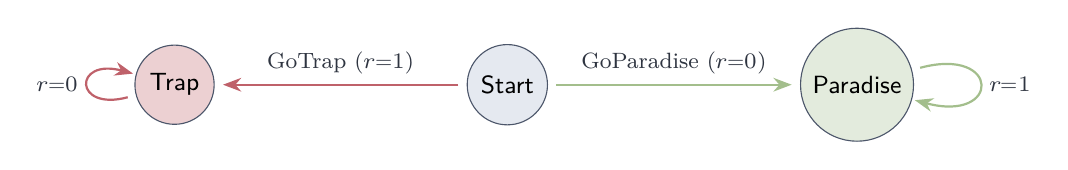
\begin{tikzpicture}[
    node distance=3.2cm,
    state/.style={draw=nord3,circle,minimum size=2em,font=\small\sffamily,fill=nord5},
    arr/.style={->,thick,>=Stealth,shorten >=3pt,shorten <=3pt}
]
\node[state,fill=nord11!30] (T) {Trap};
\node[state,right=of T] (S) {Start};
\node[state,right=of S,fill=nord14!30] (P) {Paradise};

\draw[arr,nord11] (S) -- node[above,font=\footnotesize,color=nord0] {GoTrap ($r{=}1$)} (T);
\draw[arr,nord14] (S) -- node[above,font=\footnotesize,color=nord0] {GoParadise ($r{=}0$)} (P);
\draw[arr,nord11] (T) edge[loop left] node[left,font=\footnotesize,color=nord0] {$r{=}0$} (T);
\draw[arr,nord14] (P) edge[loop right] node[right,font=\footnotesize,color=nord0] {$r{=}1$} (P);
\end{tikzpicture}}
\end{center}

GoParadise sacrifices the immediate reward ($0$ vs~$1$) but leads to Paradise (reward~$1$ forever).  GoTrap grabs the immediate reward but leads to Trap (reward~$0$ forever).

\textbf{CoinductiveHomomorphism:} $\mathit{value}(\text{Trap}) = [0,0,\ldots] \le_s [1,1,\ldots] = \mathit{value}(\text{Paradise})$ \checkmark

\textbf{CoindHomo:} Cannot rank GoTrap $\le$ GoParadise (head requires $1 \le 0$). Cannot rank GoParadise $\le$ GoTrap either (tail comparison yields $1 \le 0$ at the head of the successor streams). The actions are \emph{incomparable}---even though one is clearly better.

Full proof: \fpath{src/CSHRL/Tasks/Verified/BinarySacrifice.agda}

\subsection{Skill Investment: Multi-Stage Sacrifice}

A chain of investment decisions where training sacrifices immediate reward to advance:

\begin{center}
\resizebox{\textwidth}{!}{%
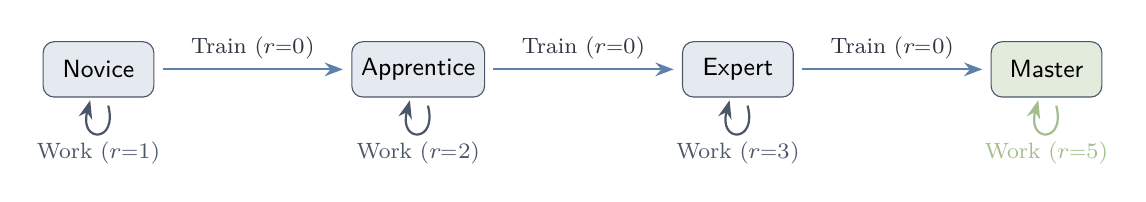
\begin{tikzpicture}[
    state/.style={draw=nord3,rounded corners,minimum size=2em,font=\small\sffamily,fill=nord5,minimum width=4em},
    arr/.style={->,thick,>=Stealth,shorten >=3pt,shorten <=3pt}
]
\node[state] (N) {Novice};
\node[state,right=2.5cm of N] (A) {Apprentice};
\node[state,right=2.5cm of A] (E) {Expert};
\node[state,right=2.5cm of E,fill=nord14!30] (M) {Master};

\draw[arr,nord10] (N) -- node[above,font=\footnotesize,color=nord0] {Train ($r{=}0$)} (A);
\draw[arr,nord10] (A) -- node[above,font=\footnotesize,color=nord0] {Train ($r{=}0$)} (E);
\draw[arr,nord10] (E) -- node[above,font=\footnotesize,color=nord0] {Train ($r{=}0$)} (M);

\draw[arr,nord3] (N) edge[loop below] node[below,font=\footnotesize,color=nord3] {Work ($r{=}1$)} (N);
\draw[arr,nord3] (A) edge[loop below] node[below,font=\footnotesize,color=nord3] {Work ($r{=}2$)} (A);
\draw[arr,nord3] (E) edge[loop below] node[below,font=\footnotesize,color=nord3] {Work ($r{=}3$)} (E);
\draw[arr,nord14] (M) edge[loop below] node[below,font=\footnotesize,color=nord14] {Work ($r{=}5$)} (M);
\end{tikzpicture}}
\end{center}

The capability profiles (value streams) form a clean progression:
\[
\begin{aligned}
\text{Master:}\quad     &[5, 5, 5, 5, \ldots] \\
\text{Expert:}\quad     &[3, 5, 5, 5, \ldots] \\
\text{Apprentice:}\quad &[2, 3, 5, 5, \ldots] \\
\text{Novice:}\quad     &[1, 2, 3, 5, \ldots]
\end{aligned}
\]

\noindent These are \emph{not trajectories}.  Consider the Apprentice profile~$[2, 3, 5, \ldots]$: the~$2$ at depth~$0$ comes from Working (best immediate reward), the~$3$ at depth~$1$ comes from Training to Expert \emph{then} Working (a different action plan), and the~$5$ at depth~$2$ comes from Training twice to Master then Working (yet another plan).  Each entry independently records the best the agent \emph{could} achieve at that depth.  No single action sequence produces the stream $[2, 3, 5, \ldots]$.

CoinductiveHomomorphism compares these profiles: Train's successor (Expert, profile~$[3,5,5,\ldots]$) pointwise dominates Work's successor (Apprentice, profile~$[2,3,5,\ldots]$).  The sacrifice---Train's immediate reward of~$0$ versus Work's~$2$---does not appear in the successor profiles, because the profiles record reachable capability, not incurred cost.

CoindHomo fails at every level: Work's immediate reward always exceeds Train's, so the action-value streams are pointwise incomparable.

Full proof: \fpath{src/CSHRL/Tasks/Verified/SkillInvestment.agda}

\subsection{Preparation Dilemma: Cyclic Dynamics}

A structurally different pattern with regression and context-dependent optimal actions:

\begin{center}
\resizebox{\textwidth}{!}{%
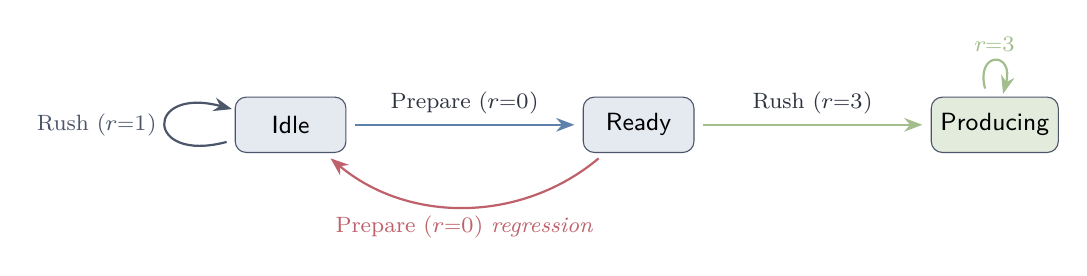
\begin{tikzpicture}[
    node distance=3cm,
    state/.style={draw=nord3,rounded corners,minimum size=2em,font=\small\sffamily,fill=nord5,minimum width=4em},
    arr/.style={->,thick,>=Stealth,shorten >=3pt,shorten <=3pt}
]
\node[state] (I) {Idle};
\node[state,right=of I] (R) {Ready};
\node[state,right=of R,fill=nord14!30] (P) {Producing};

% forward transitions, labels above
\draw[arr,nord10] (I) -- node[above,font=\footnotesize,color=nord0] {Prepare ($r{=}0$)} (R);
\draw[arr,nord14] (R) -- node[above,font=\footnotesize,color=nord0] {Rush ($r{=}3$)} (P);

% self loops kept off the centre line: Idle to the left, Producing above
\draw[arr,nord3] (I) edge[loop left] node[left,font=\footnotesize,color=nord3] {Rush ($r{=}1$)} (I);
\draw[arr,nord14] (P) edge[loop above] node[above,font=\footnotesize,color=nord14] {$r{=}3$} (P);

% regression curves below, label below
\draw[arr,nord11] (R) to[bend left=40] node[below,font=\footnotesize,color=nord11] {Prepare ($r{=}0$) \emph{regression}} (I);
\end{tikzpicture}}
\end{center}

\noindent At Idle, the optimal action is Prepare (sacrifice now for readiness).  At Ready, the optimal action flips to Rush (capitalize on preparation).  Over-preparing at Ready sends the agent \emph{back} to Idle---a regression penalty.

Value streams: $\text{Producing} = \text{Ready} = [3,3,3,\ldots]$, $\text{Idle} = [1,3,3,\ldots]$.

CoinductiveHomomorphism handles the context-dependent ranking: Prepare $>$ Rush at Idle (successor quality improves), Rush $>$ Prepare at Ready (successor quality improves).

CoindHomo cannot rank the actions at Idle in \emph{either} direction:
\begin{itemize}
\item Forward (Rush $\le$ Prepare): head requires $1 \le 0$---absurd.
\item Reverse (Prepare $\le$ Rush): head is $0 \le 1$ (ok), but the tail requires $\mathit{value}(\text{Ready}) \le_s \mathit{value}(\text{Idle})$, which fails at the head: $3 \le 1$---absurd.
\end{itemize}

Full proof: \fpath{src/CSHRL/Tasks/Verified/PreparationDilemma.agda}

%%%%%%%%%%%%%%%%%%%%%%%%%%%%%%%%%%%%%%%%%%%%%%%%%%%%%%%%%%%%%%%%%%%%%%%%%%%%%%%
% PART VII: SUBSUMPTION
%%%%%%%%%%%%%%%%%%%%%%%%%%%%%%%%%%%%%%%%%%%%%%%%%%%%%%%%%%%%%%%%%%%%%%%%%%%%%%%

\section{Relationship to Classical Reinforcement Learning}\label{sec:subsumes}

The value streams compared by CoinductiveHomomorphism are computed from the actual environment dynamics by the \texttt{solve} function---they are ground truth, not estimates.  If the environment terminates (absorbing states with zero reward), the value streams reflect that.  If the environment is infinite, the streams extend accordingly.  The horizon is not a parameter of the condition; it is encoded in the dynamics.

\subsection{Relationship to Classical Optimality}

Both conditions are sound with respect to classical objectives, and each subsumes a different one.

\paragraph{CoindHomo subsumes discounted return.}  The action-value condition compares the \emph{full} action-value streams, whose head is the immediate reward.  Pointwise dominance at every position implies that the cumulative sum---at every finite horizon---is at least as large for the better-ranked action.  Since discounted return is a positively weighted sum, action-value dominance implies discounted-return dominance for every $\gamma \in [0,1)$: any policy optimal under CoindHomo is optimal under every discounted-return criterion.

\paragraph{CoinductiveHomomorphism subsumes successor return.}  The successor condition compares successor value streams---the accumulated reward \emph{from the state the action leads to}.  The verified theorem:

\begin{code}[hide]
  iter-head : ℕ → StreamR → Reward
  iter-head zero    s = head s
  iter-head (suc n) s = iter-head n (tail s)

  PointwiseDominance : StreamR → StreamR → Set
  PointwiseDominance x y = ∀ n → iter-head n x ≤ᵣ iter-head n y

  ≤ₛ-to-pointwise : ∀ {x y} → x ≤ₛ y → PointwiseDominance x y
  ≤ₛ-to-pointwise p zero    = head≤ p
  ≤ₛ-to-pointwise p (suc n) = ≤ₛ-to-pointwise (tail≤ p) n
\end{code}

\begin{code}[hide]
module CoreWithArithmetic
  (State Action Reward : Set)
  (step                : State → Action → State × Reward)
  (_≤ᵣ_                : Reward → Reward → Set)
  (max                 : Reward → Reward → Reward)
  (bottom              : Reward)
  (all-actions         : List Action)
  (_+ᵣ_                : Reward → Reward → Reward)
  (≤ᵣ-refl             : ∀ {r} → r ≤ᵣ r)
  (+ᵣ-mono-≤           : ∀ {a b c d} → a ≤ᵣ b → c ≤ᵣ d → (a +ᵣ c) ≤ᵣ (b +ᵣ d))
  where

  open Core State Action Reward step _≤ᵣ_ max bottom all-actions public

  pointwise-tail : ∀ {x y} → PointwiseDominance x y → PointwiseDominance (tail x) (tail y)
  pointwise-tail pw n = pw (suc n)

  partial-sum : ℕ → StreamR → Reward
  partial-sum zero    _ = bottom
  partial-sum (suc n) s = head s +ᵣ partial-sum n (tail s)

  partial-sum-mono : ∀ N x y → PointwiseDominance x y →
                     partial-sum N x ≤ᵣ partial-sum N y
  partial-sum-mono zero _ _ _ = ≤ᵣ-refl
  partial-sum-mono (suc n) x y pw =
    +ᵣ-mono-≤ (pw zero) (partial-sum-mono n (tail x) (tail y) (pointwise-tail pw))
\end{code}

\begin{code}[hide]
  subsumes-successor-return : (ch : CoinductiveHomomorphism) →
    ∀ s a b N →
    CoinductiveHomomorphism._≤ₐ_ ch s a b →
    partial-sum N (successor-value s a) ≤ᵣ
    partial-sum N (successor-value s b)
  subsumes-successor-return ch s a b N p =
    partial-sum-mono N _ _ (≤ₛ-to-pointwise
      (CoinductiveHomomorphism.preserves ch a b s p))
\end{code}

\noindent The top-ranked action leads to the state with the highest accumulated reward at every finite horizon.  This is successor return dominance: the better-ranked action places the agent in a strictly better position.

\subsection{CoinductiveHomomorphism Is Sound Where Classical Methods Can Fail}

CoindHomo refuses to rank in sacrifice environments, remaining conservative.  By contrast, the CoinductiveHomomorphism condition continues to produce correct rankings, while classical discounted methods can actively select the \emph{wrong} action in exactly these cases.  To make the contrast concrete, we examine Q-learning---the workhorse algorithm of model-free reinforcement learning~\cite{Sutton2018}.  Q-learning maintains a table of \emph{Q-values}, $Q(s, a)$, estimating the expected discounted return of taking action~$a$ in state~$s$ and acting optimally thereafter.  These estimates are updated via the Bellman equation:
\[
Q(s, a) \;\leftarrow\; r(s, a) \;+\; \gamma \cdot \max_{a'} Q(s', a')
\]
where $r(s,a)$ is the immediate reward, $s'$ is the successor state, and $\gamma \in [0, 1)$ is the discount factor.  The agent then selects the action with the highest Q-value: $\pi(s) = \arg\max_a Q(s, a)$.  Under standard conditions, Q-learning converges to the optimal Q-values, and the greedy policy is optimal \emph{for the discounted objective}.  The problem, as we now show, is that the discounted objective itself can be wrong.

In sacrifice environments, Q-learning can converge to a suboptimal policy---not because the algorithm fails, but because the discount factor distorts the objective it optimizes.  We demonstrate this concretely on the binary sacrifice MDP.

\paragraph{The verified ground truth.}
The \texttt{solve} function computes the optimal reward at each depth from the actual environment dynamics:
\[
\begin{aligned}
\text{solve}(\text{Paradise}, n) &= 1 \quad \text{for all } n \\
\text{solve}(\text{Trap}, n) &= 0 \quad \text{for all } n
\end{aligned}
\]
These are machine-verified facts, not estimates.  Paradise yields reward~$1$ at every future depth; Trap yields~$0$.  The accumulated reward from Paradise at horizon~$N$ is~$N$; from Trap it is~$0$.

\paragraph{The Q-value computation.}
The Bellman equation gives Q-learning's converged values at state Start:
\[
\begin{aligned}
Q(\text{Start}, \text{GoTrap})     &= \underbrace{1}_{\text{immediate}} + \gamma \cdot \underbrace{0}_{\textstyle V(\text{Trap})} = 1 \\[6pt]
Q(\text{Start}, \text{GoParadise}) &= \underbrace{0}_{\text{immediate}} + \gamma \cdot \underbrace{\tfrac{1}{1-\gamma}}_{\textstyle V(\text{Paradise})} = \tfrac{\gamma}{1-\gamma}
\end{aligned}
\]
For $\gamma < \tfrac{1}{2}$, we have $\tfrac{\gamma}{1-\gamma} < 1$, so Q-learning selects GoTrap---the action whose successor state has accumulated reward~$0$ at every horizon---over GoParadise, whose successor state has accumulated reward~$N$ at horizon~$N$.

The discount factor $\gamma$ geometrically suppresses $V(\text{Paradise})$, which is the only term that carries the evidence of Paradise's superiority.  When $\gamma$ is small enough, the suppression is sufficient to make a state worth $[1,1,1,\ldots]$ appear less valuable than a state worth $[0,0,0,\ldots]$.

\paragraph{The verified conclusion.}
We prove in Agda (\fpath{src/CSHRL/Analysis/QLearningFailure.agda}) the conjunction of two facts:
\begin{enumerate}
\item \textbf{Tactical:} $r(\text{Start}, \text{GoParadise}) \le r(\text{Start}, \text{GoTrap})$ --- GoTrap has the higher immediate reward.
\item \textbf{Strategic:} For every horizon~$N$, the accumulated reward from GoParadise's successor exceeds GoTrap's:
\[
\sum_{i=0}^{N-1} \text{solve}(\text{Trap}, i) \;\le\; \sum_{i=0}^{N-1} \text{solve}(\text{Paradise}, i)
\]
\end{enumerate}
Together: Q-learning with $\gamma < \tfrac{1}{2}$ selects the action with the higher immediate reward and the strictly inferior successor state.  The discount factor is the mechanism by which the tactical advantage overrides the strategic one.

\paragraph{Deeper sacrifice chains.}
The Skill Investment chain sharpens the point.  Q-learning requires $\gamma > (1/5)^{1/3} \approx 0.585$ to identify the optimal training path.  Below this threshold, it converges to the policy of working at Novice forever---earning~$1$ per step while a three-step investment would yield~$5$ per step permanently.  CoinductiveHomomorphism identifies the training path regardless: the successor state quality is strictly better at every depth, and the environment dynamics confirm it.

\subsection{CoindHomo as the Conservative Special Case}

CoindHomo is best understood as a deliberate conservative restriction of the CoinductiveHomomorphism condition.  One might prefer it precisely when its extra demand---that immediate rewards also respect the ranking---is desirable: it bundles tactical and strategic soundness, so its rankings are compatible with existing discounted-return theory and algorithms without further argument.  In aligned environments (Section~\ref{sec:landscape}), where the two conditions coincide, this comes for free, and CoinductiveHomomorphism inherits CoindHomo's full subsumption of classical RL.

The restriction has a cost.  In sacrifice environments CoindHomo cannot rank the actions at all---the action-value streams are pointwise incomparable---whereas CoinductiveHomomorphism still identifies the better successor state, which the environment dynamics validate.  CoindHomo refuses to rank when immediate reward conflicts with the future; CoinductiveHomomorphism resolves the conflict in favor of successor state quality.

%%%%%%%%%%%%%%%%%%%%%%%%%%%%%%%%%%%%%%%%%%%%%%%%%%%%%%%%%%%%%%%%%%%%%%%%%%%%%%%
% PART VIII: STREAM ISOMORPHISM
%%%%%%%%%%%%%%%%%%%%%%%%%%%%%%%%%%%%%%%%%%%%%%%%%%%%%%%%%%%%%%%%%%%%%%%%%%%%%%%

\section{Stream Isomorphism}\label{sec:stream-iso}

We defined stream dominance coinductively: $x \le_s y$ holds if the heads compare and the tails recursively compare.  This definition is equivalent to pointwise dominance at every timestep.  The forward direction follows by unfolding the definition.  The converse is established by coinduction: if $x_n \le_r y_n$ for every~$n$, then both \texttt{head≤} and \texttt{tail≤} hold, hence $x \le_s y$.

\begin{code}[hide]
module IsoSketch
  (Reward : Set)
  (_≤ᵣ_ : Reward → Reward → Set)
  where
  
  open import Data.Nat using (ℕ; zero; suc)
  
  record StreamR : Set where
    coinductive
    field head : Reward
          tail : StreamR
  open StreamR public
  
  iter-head : ℕ → StreamR → Reward
  iter-head zero s = head s
  iter-head (suc n) s = iter-head n (tail s)
  
  PointwiseDominance : StreamR → StreamR → Set
  PointwiseDominance x y = ∀ n → iter-head n x ≤ᵣ iter-head n y

  record _≤ₛ_ (x y : StreamR) : Set where
    coinductive
    field head≤ : head x ≤ᵣ head y
          tail≤ : tail x ≤ₛ tail y
  open _≤ₛ_ public
  
  pointwise-tail : ∀ {x y} → PointwiseDominance x y → PointwiseDominance (tail x) (tail y)
  pointwise-tail pw n = pw (suc n)
\end{code}

\begin{code}[hide]
  pointwise-to-≤ₛ : ∀ {x y} → PointwiseDominance x y → x ≤ₛ y
  head≤ (pointwise-to-≤ₛ pw) = pw zero
  tail≤ (pointwise-to-≤ₛ pw) = pointwise-to-≤ₛ (pointwise-tail pw)
\end{code}

This equivalence has two direct consequences.  First, it confirms that the coinductive formulation precisely captures dominance at every future depth.  Second, it justifies the completeness of the Finder: because the Finder decides rankings via finite trace comparison, and trace dominance at all depths implies coinductive stream dominance, every ranking returned by the Finder satisfies the coinductive condition.

The isomorphism holds for both successor-value and action-value streams, and therefore supports both CoinductiveHomomorphism and CoindHomo.  The full proof is in \fpath{src/appendix/StreamIsomorphism.agda}.

%%%%%%%%%%%%%%%%%%%%%%%%%%%%%%%%%%%%%%%%%%%%%%%%%%%%%%%%%%%%%%%%%%%%%%%%%%%%%%%
% PART VIII: THE ALGORITHM
%%%%%%%%%%%%%%%%%%%%%%%%%%%%%%%%%%%%%%%%%%%%%%%%%%%%%%%%%%%%%%%%%%%%%%%%%%%%%%%

\section{The Finder Algorithm}\label{sec:finder}

The preceding sections established what an optimal ranking \emph{is}.  We now turn to how to \emph{compute} one.  The Finder algorithm uses lexicographic trace comparison and requires no discount factor.

\begin{code}[hide]
module Finder
  (State Action Reward : Set)
  (step                : State → Action → State × Reward)
  (_≤?_                : Reward → Reward → Bool)
  (default-action      : Action)
  (all-actions         : List Action)
  where

  open import Data.List using (List; map)

  Trace : Set
  Trace = List Reward
\end{code}

\subsection{Lexicographic Comparison}

Compare traces element-by-element---the first difference decides:

\begin{code}[hide]
  _≤ₜ_ : Trace → Trace → Bool
  []       ≤ₜ []       = true
  []       ≤ₜ (_ ∷ _)  = true
  (_ ∷ _)  ≤ₜ []       = false
  (r₁ ∷ t₁) ≤ₜ (r₂ ∷ t₂) =
    if r₁ ≤? r₂ then
      if r₂ ≤? r₁ then (t₁ ≤ₜ t₂)
      else true
    else false
\end{code}

\noindent Unlike summation (which discards timing information), lexicographic comparison preserves it: a trace $[10, -5]$ dominates $[0, 5]$ because $10 > 0$ at step~$0$, regardless of subsequent elements.

\subsection{Trace Evaluation}

Given the comparator, we need the traces themselves.  For a deterministic MDP, the trace of action~$a$ at state~$s$ to depth~$k$ is the finite prefix of the reward stream: take action~$a$, record the reward, then act optimally (according to all actions, greedily at each step) for the remaining~$k{-}1$ steps.  \texttt{best-trace} computes this optimal continuation; \texttt{trace-action} prepends the immediate reward of a specific action:

\begin{code}[hide]
  mutual
    best-trace : State → ℕ → Trace
    best-trace s zero    = []
    best-trace s (suc k) =
      let outcomes = map (λ a → trace-action s a k) all-actions
      in max-trace outcomes

    trace-action : State → Action → ℕ → Trace
    trace-action s a k =
      let (s' , r) = step s a
          future   = best-trace s' k
      in r ∷ future

    max-trace : List Trace → Trace
    max-trace []       = []
    max-trace (t ∷ ts) = max-helper t ts

    max-helper : Trace → List Trace → Trace
    max-helper current [] = current
    max-helper current (t ∷ ts) =
      if current ≤ₜ t
      then max-helper t ts
      else max-helper current ts
\end{code}

\subsection{The Ranking Finder}

With traces and a comparator in hand, producing a ranking is straightforward: compute each action's trace at the desired depth, then sort by lexicographic dominance.  The head of the sorted list is the optimal action; the full list is the total ranking used by the adaptation layer (\S\ref{sec:adaptation}).

\begin{code}[hide]
  insert : (Action × Trace) → List (Action × Trace) → List (Action × Trace)
  insert x [] = x ∷ []
  insert (a₁ , t₁) ((a₂ , t₂) ∷ xs) =
    if t₂ ≤ₜ t₁
    then (a₁ , t₁) ∷ (a₂ , t₂) ∷ xs
    else (a₂ , t₂) ∷ insert (a₁ , t₁) xs

  sort-scored : List (Action × Trace) → List (Action × Trace)
  sort-scored [] = []
  sort-scored (x ∷ xs) = insert x (sort-scored xs)

  find-ranking : State → ℕ → List Action
  find-ranking s k =
    let scored = map (λ a → (a , trace-action s a k)) all-actions
        sorted = sort-scored scored
    in map proj₁ sorted

  find-policy : State → ℕ → Action
  find-policy s k =
    let ranking = find-ranking s k
    in head-default ranking
    where
      head-default : List Action → Action
      head-default []      = default-action
      head-default (x ∷ _) = x
\end{code}

\noindent No discount factor is required.  Standard RL needs $\gamma < 1$ to ensure convergence of the sum; here we compare structure directly, and the lexicographic order is well-defined at any depth.

\subsection{Serving Both Conditions}

The Finder as defined above computes \texttt{trace-action}---whose head is the immediate reward and whose tail is the optimal future.  This directly serves \textbf{CoindHomo}: action-value traces are the finite approximations of action-value streams.

For \textbf{CoinductiveHomomorphism}, the relevant comparison is between \emph{successor-value traces}---the optimal future from the state reached by each action, \emph{excluding} the immediate reward.  The adaptation is a one-line change: instead of \texttt{r~∷~future}, use \texttt{future} alone.  Equivalently, compare \texttt{tail(trace-action~s~a~k)} for each action.

In aligned environments (Section~\ref{sec:landscape}), both comparisons yield the same ranking.  In sacrifice environments, the action-value trace may be incomparable (the head reversal prevents lexicographic dominance), while the successor-value trace correctly identifies the better successor state.  The Stream Isomorphism (\S\ref{sec:stream-iso}) guarantees that trace dominance at all depths implies coinductive stream dominance---for whichever stream variant is used.

\section{Environment Classes: Modularity Without Postulates}\label{sec:env-classes}

The Finder produces rankings; the Stream Isomorphism connects them to coinductive stream dominance.  But each task still needs its own bridge lemma---a potentially tedious and error-prone process.  The \textbf{Environment Class} (EC) abstraction eliminates this boilerplate.  Rather than proving preservation from scratch for each task, we factor out common structure into reusable modules.

\subsection{Parameterized Modules}

Without environment classes, every task would need its own Finder, trace-to-stream bridge, and preservation skeleton---duplication that also raises trust questions about which parts are verified.  Environment classes instead provide \textbf{verified infrastructure} that task instances inherit: a task author fills in a parameter record (\texttt{ECParameters}: types, step function, reward order with decidability and extrema, and finiteness witnesses), and the class automatically supplies the Finder, trace types, stream bridges, and proof scaffolding (full implementation in \fpath{src/CSHRL/EnvironmentClass/}).

\begin{code}[hide]
module FiniteDeterministicMDPSignature where
  open import Data.Unit using (⊤)
  open import Data.Empty using (⊥)
\end{code}

\begin{code}[hide]
  record ECParameters : Set₁ where
    field
      State Action Reward : Set
      step      : State → Action → State × Reward
      _≤ᵣ_      : Reward → Reward → Set
      _≤?_      : (r s : Reward) → Dec (r ≤ᵣ s)
      ≤ᵣ-refl   : ∀ {r} → r ≤ᵣ r
      max       : Reward → Reward → Reward
      bottom    : Reward
      all-actions    : List Action
      default-action : Action
      horizon   : ℕ
\end{code}

\begin{code}[hide]
  module ECProvides (P : ECParameters) where
    open ECParameters P
    
    Trace : Set
    Trace = List Reward
    
    _≤ₜ_ : Trace → Trace → Set
    []       ≤ₜ []       = ⊤
    []       ≤ₜ (_ ∷ _)  = ⊤
    (_ ∷ _)  ≤ₜ []       = ⊥
    (r₁ ∷ t₁) ≤ₜ (r₂ ∷ t₂) = (r₁ ≤ᵣ r₂) × ((r₂ ≤ᵣ r₁) → t₁ ≤ₜ t₂)
\end{code}

\noindent The fields divide into a \emph{domain} group (\texttt{State}, \texttt{Action}, \texttt{step}), an \emph{algebraic} group (the ordered reward structure \texttt{\_$\le$ᵣ\_}, \texttt{\_$\le$?\_}, \texttt{max}, \texttt{bottom}), and an \emph{enumeration} group (\texttt{all-actions}, \texttt{horizon}) supplying the finiteness witnesses the Finder needs.  From these, the EC derives the trace orderings, the Finder, the ranking relation, the trace-to-stream bridge, and---for specialised ECs---a full \texttt{CoindHomo}.

\begin{code}[hide]
  -- AUTOMATICALLY PROVIDED by the EC:
  -- • Trace type and orderings (_≤ₜ_, _≤ₜᵇ_)
  -- • Finder algorithm (best-trace, find-ranking, find-policy)
  -- • Ranking relation (_ranks_≤_)
  -- • Trace-to-stream bridge infrastructure (trace-≤ₜ-head)
  -- • Stream reflexivity (≤ₛ-refl)
  -- • Full CoindHomo (for specialised ECs like CombinatorialPlacementMDP)
\end{code}

\subsection{What Task Instances Must Provide}\label{sec:task-provide}

For the general \textbf{FiniteDeterministicMDP}, a task supplies the domain (\texttt{State}, \texttt{Action}, \texttt{step}) plus a direct proof that the Finder's ranking preserves action-value ordering.  The specialised \textbf{CombinatorialPlacementMDP}\label{sec:cpmdp} (for placement problems such as N-Queens, Sudoku, Graph Coloring) reduces this burden further; full implementation in \fpath{src/CSHRL/EnvironmentClass/CombinatorialPlacementMDP.agda}.

\begin{code}[hide]
module CombinatorialPlacementSignature where
\end{code}

\begin{code}[hide]
  record PlacementParameters : Set₁ where
    field
      Config : Set
      Action : Set
      is-dead   : Config → Bool
      is-solved : Config → Bool
      place : Config → Action → Config
      solved-reward : ℕ
      all-actions : List Action
      default-action : Action
      horizon : ℕ

  data PlacementState (Config : Set) : Set where
    Ongoing : Config → PlacementState Config
    Dead    : PlacementState Config
    Solved  : Config → PlacementState Config
\end{code}

\noindent The three constructors model a placement problem's life cycle: \texttt{Ongoing} wraps an active configuration, \texttt{Dead} is an absorbing failure (stream~$[0,0,\ldots]$), and \texttt{Solved} a completed configuration (stream~$[R,R,\ldots]$).  Any path reaching Solved thus dominates any path reaching Dead at every timestep---exactly the coinductive order's requirement.  The EC factors preservation into three reusable layers---\texttt{WithAbsorbingLemmas} (absorbing-state domination), \texttt{WithBinaryStructure} (every value is $0$ or $R$, with monotonicity), and \texttt{WithTraceBridge} (horizon sufficiency $\Rightarrow$ full \texttt{CoindHomo})---so the task author supplies at most four simple ingredients while the machinery handles the finite-trace-to-infinite-stream bridge.

\paragraph{Validation: 8-Queens.}
The \texttt{Queens8} module (\fpath{src/CSHRL/Tasks/Verified/Queens8.agda}) instantiates the EC with \texttt{--safe} and zero postulates: discharging \texttt{solve-horizon-suf} and opening \texttt{WithTraceBridge} yields a complete \texttt{CoindHomo} over a combinatorial search space ($8^8 = 16{,}777{,}216$ candidate placements) where direct stream enumeration is infeasible.  More broadly, verified tasks (TwoState, Queens1, Queens8) carry no postulates; classic tasks may postulate hard-to-formalise properties while keeping the \emph{structural} preservation proof verified; and new tasks inherit all machinery by instantiating the parameter record.

\begin{figure}[H]
\centering
\begin{tikzpicture}[
    node distance=0.8cm and 1.0cm,
    box/.style={draw,rounded corners,minimum height=2.0em,minimum width=5em,align=center,font=\footnotesize},
    groupbox/.style={draw,rounded corners,inner sep=0.3cm,fill=white},
    smallbox/.style={rounded corners,minimum height=1.4em,minimum width=3.5em,align=center,font=\tiny,fill=nord13!25},
    stochbox/.style={rounded corners,minimum height=1.4em,minimum width=3.5em,align=center,font=\tiny,fill=nord14!35},
    inherit/.style={->,thick,>=Stealth,dashed},
    arr/.style={->,>=Stealth}
]
\node[box,fill=nord9!20] (core) {Core.agda\\(Theory)};
\node[box,fill=nord15!20,right=3.5cm of core] (stoch) {Core/Stochastic\\(Giry monad)};

\node[box,fill=nord7!25,below left=1.0cm and 1.5cm of core] (fdmdp) {FiniteDeterministic\\MDP};
\node[box,fill=nord7!25,below=1.0cm of core] (cpmdp) {Combinatorial\\PlacementMDP};
\node[box,fill=nord15!30,below=1.0cm of stoch] (smdp) {Stochastic\\FiniteMDP};

\node[groupbox,below=0.8cm of fdmdp] (fdtasks) {
  \begin{tikzpicture}
    \node[smallbox] (t1) {TwoState};
    \node[smallbox,right=0.1cm of t1] (t2) {GridWorld};
    \node[smallbox,below=0.1cm of t1] (t3) {KeyTreasure};
    \node[smallbox,right=0.1cm of t3] (t4) {\ldots};
  \end{tikzpicture}
};

\node[groupbox,below=0.8cm of cpmdp] (cptasks) {
  \begin{tikzpicture}
    \node[smallbox] (q1) {Queens1};
    \node[smallbox,right=0.1cm of q1] (q8) {Queens8};
  \end{tikzpicture}
};

\node[groupbox,below=0.8cm of smdp] (stasks) {
  \begin{tikzpicture}
    \node[stochbox] (s1) {CoinFlip};
    \node[stochbox,right=0.1cm of s1] (s2) {GamblersRuin};
    \node[stochbox,below=0.1cm of s1] (s3) {RandomWalk};
    \node[stochbox,right=0.1cm of s3] (s4) {BiasedBandit};
  \end{tikzpicture}
};

\draw[inherit] (core) -- (fdmdp);
\draw[inherit] (core) -- (cpmdp);
\draw[inherit] (stoch) -- (smdp);

\draw[arr] (fdmdp) -- (fdtasks);
\draw[arr] (cpmdp) -- (cptasks);
\draw[arr] (smdp) -- (stasks);
\end{tikzpicture}
\caption{Environment class hierarchy.  Core provides theory; ECs provide reusable verification infrastructure; task groups contain domain-specific instantiations.}
\label{fig:ec-hierarchy}
\end{figure}

\section{Stochastic Extension}\label{sec:stochastic}

Everything up to this point assumes deterministic environments. Many real-world problems are inherently stochastic: a robot's actuators have noise, a card game involves shuffled decks, or a medical treatment has variable patient responses. In such environments the step function returns a probability distribution over outcomes rather than a single successor state and reward.

The classical approach to stochastic MDPs uses the Giry monad~\cite{Giry1982}, but its full generality (measurable spaces and $\sigma$-algebras) is far too heavy for constructive, decidable verification in Agda. We therefore use a \emph{finite distribution monad}: a discrete, constructive approximation that represents distributions as weighted lists. This gives exact arithmetic, decidable equality, and compatibility with Agda's termination checker while remaining expressive enough for any finite-state stochastic MDP. The monad operations (\texttt{pure}, \texttt{scale}, \texttt{>>=}) and their laws are verified in \fpath{src/CSHRL/Probability/Finite.agda}.

\subsection{Lexicographic Coinductive Comparison}

In stochastic MDPs the value at each depth is an \emph{expected} reward. The deterministic pointwise order $\leq_s$ is too strict here: if action $a$ already wins at depth 0 in expectation, demanding it also wins at every later depth would rule out many valid rankings. The appropriate notion is \emph{lexicographic coinductive comparison} ($\leq_{lex}$): compare expected heads, and recurse on the tails only when the heads are equal. This remains coinductive but lets earlier rewards break ties.

\subsection{Stochastic Coinductive Homomorphism}

We can now lift both conditions from the deterministic setting.

\begin{itemize}
\item \textbf{StochasticCoindHomo} preserves expected action-value streams lexicographically. This bundles the immediate expected reward and the expected successor quality.
\item \textbf{StochasticCoinductiveHomomorphism} preserves expected successor-value streams lexicographically. This decouples immediate reward, allowing sacrifice-pattern reasoning in stochastic environments.
\end{itemize}

The decomposition theorem (Theorem~\ref{thm:decomposition}) lifts directly: the stochastic action-value condition decomposes into expected-immediate-reward compatibility plus stochastic successor-quality preservation. The full implementation is in \fpath{src/CSHRL/Core/Stochastic.agda}, with the corresponding Environment Class in \fpath{src/CSHRL/EnvironmentClass/StochasticFiniteMDP.agda}.

All four verified stochastic examples (\texttt{CoinFlip}, \texttt{GamblersRuin}, \texttt{RandomWalk}, \texttt{BiasedBandit}) follow the same verification pattern: one action dominates in expected immediate reward (so the head obligation follows from the ranking hypothesis), while the tail obligation requires two expected heads to be equal---an absurdity discharged by the empty pattern. All four are therefore fully verified with zero postulates.

\subsection{Distributional Hierarchy}

The framework so far compares actions by their expected reward streams. Stronger distributional guarantees are available through a hierarchy of stochastic dominance relations. \textbf{First-Order Stochastic Dominance} (FOSD) requires that the cumulative distribution of one action lies everywhere below that of another at every timestep. The \textbf{Stochastic Dominance Hierarchy} generalizes this: $\text{SD}[0] = \text{FOSD}$, $\text{SD}[1] = \text{SOSD}$, $\text{SD}[2] = \text{TOSD}$, etc. Each additional level integrates the CDF and captures a broader class of utility functions while remaining verifiable.

A single FOSD verification automatically yields optimality at all higher SD levels. The complete pipeline (distribution level and stream level) is machine-verified in \fpath{src/CSHRL/Probability/FOSD.agda}, \fpath{src/CSHRL/Core/FOSD.agda}, \fpath{src/CSHRL/Probability/SD.agda}, and \fpath{src/CSHRL/Core/SD.agda}. These stronger distributional conditions align naturally with \texttt{StochasticCoindHomo}; the lexicographic \texttt{StochasticCoinductiveHomomorphism} sits outside the per-timestep hierarchy, as expected.

Pointwise dominance implies lexicographic dominance (but not conversely), and the two coincide in the deterministic case. Classical RL is subsumed via linearity of expectation.

\section{Compositional Ranking Algebra}\label{sec:compose}

As environments grow in complexity, monolithic verification becomes impractical.  Consider a warehouse robot that must navigate (an MDP with 20~states) \emph{and} pick items (an MDP with 50~configurations).  Verifying the product MDP ($20 \times 50 = 1000$ states, $O(|A|^2)$ pairs per state) is far more expensive than verifying each component independently.  The Compositional Ranking Algebra proves that verified rankings \emph{compose}---enabling a ``divide and conquer'' strategy: verify navigation and picking separately, then combine.

The foundation is that \texttt{prefix-sum} is a \emph{linear operator}, so the SD$[k]$ ordering (built from iterated prefix sums) is closed under distribution concatenation (\texttt{SD-++}) and non-negative scaling (\texttt{SD-scale})---both one-line proofs by monotonicity.  A \texttt{VerifiedRanking} bundles a ranking with a machine-checked proof that it preserves SD$[k]$ at every state and timestep, and the algebra provides five verified operations that combine \texttt{VerifiedRanking}s with \emph{zero} additional proof burden: hierarchy subsumption ($k \to k{+}1$), product composition (\texttt{++-product}), convolution product (\texttt{conv-product}, for additive-reward products, via discrete Abel summation), sum composition (disjoint environments), and scaling.  They compose freely---e.g. \texttt{scaled-product~c~vr₁~vr₂}---enabling divide-and-conquer verification of multi-component MDPs (full implementation in \fpath{src/CSHRL/Probability/Compose.agda}, \fpath{src/CSHRL/Core/Compose.agda}).

\section{Verified State Abstraction}\label{sec:abstraction}

Everything so far applies to finite MDPs where the state space can be enumerated.  But many real-world problems have infinite or very large state spaces---a robot's continuous position, a game with billions of configurations.  Verified state abstraction bridges this gap: verify a ranking on a small, finite \emph{abstract} system, then lift it to the full concrete system.

A \texttt{StateAbstraction} bundles three components:

\begin{itemize}
\item \textbf{project}: $\text{Concrete} \to \text{Abstract}$---collapses concrete states to abstract classes.
\item \textbf{embed}: $\text{Abstract} \to \text{Concrete}$---selects a representative for each class.
\item \textbf{section}: $\texttt{project} \circ \texttt{embed} = \text{id}$---the representatives are consistent.
\end{itemize}

\noindent No finiteness assumption is placed on \texttt{Concrete}: it can be $\mathbb{N}$, $\mathbb{R}^n$, or any type in \texttt{Set}.

\subsection{The Lifting Theorem}

The central result is \texttt{abstract-lift}:

\begin{quote}
\emph{Given a state abstraction and a proof that the marginal reward function is constant within each abstract class (marginal-invariance), any \texttt{VerifiedRanking} on the abstract system lifts to a \texttt{VerifiedRanking} on the full concrete system.}
\end{quote}

\noindent This is the standard model-irrelevance condition from the state abstraction literature \cite{Li2006}, but formalized constructively in Agda with a machine-checked proof.  The verification cost is $O(|\text{Abstract}|)$ regardless of the concrete space's cardinality.

Three composition operators extend the framework: \texttt{product-abstraction} (component-wise), \texttt{compose-abstraction} (chaining two-level abstractions $C \xrightarrow{\alpha_1} M \xrightarrow{\alpha_2} A$), and \texttt{abstract-conv-product} (the full pipeline: abstract each component, verify FOSD abstractly, compose via convolution, lift to the concrete product).  Validated postulate-free on infinite-state environments---Regional Policy ($\mathbb{N}$ states), Three-Zone ($\mathbb{N}$ states), and CartPole ($\mathbb{N}^4$ discretized, angle-based abstraction).  Full implementation: \fpath{src/CSHRL/Core/Abstraction.agda}.

\section{Learning as Symmetry Restoration}\label{sec:learning}

The Finder computes rankings at a fixed depth. Real learning, however, is incremental: the agent observes samples, detects violations of the homomorphism condition, and restores them.

A \emph{violation} occurs when the current ranking at a state disagrees with the ground-truth comparator (instantiated by the Finder at the current depth). The repair is a single transposition: swap the two actions so the better one precedes the worse one. Each swap fixes exactly one violated pair without disturbing unrelated pairs. Because transpositions generate the symmetric group $S_{|\mathcal{A}|}$ (\S\ref{sec:formal}), repeated swapping corresponds to walking through the space of total rankings until the environment's stream order is restored.

Formally, a violation records the state, the pair of actions, and the depth at which the disagreement was found. The fix is to apply the transposition in the ranking.

\begin{theorem}[Swap Monotonicity]
Let $v$ be a violation with actions $(\textit{better}, \textit{worse})$. After swapping: (1)~the violated pair is correctly ordered; (2)~unrelated pairs are unchanged; (3)~the total number of violations decreases by at least~$1$.
\end{theorem}

Since each swap strictly decreases the violation count and the count is non-negative, the process terminates. The worst-case bound is
\[
\text{max-violations} \leq |S| \times \binom{|\mathcal{A}|}{2} = |S| \times \frac{|\mathcal{A}|(|\mathcal{A}|-1)}{2}.
\]

The \texttt{ConvergenceTheorem} packages the full guarantee: given a valid violation finder and a sound ground-truth oracle, iterated swapping from any initial ranking reaches zero violations in at most \texttt{max-violations} steps. All proofs are in \fpath{src/CSHRL/Learning/Base.agda}.

\begin{remark}[Full-ranking learning dissolves the exploration/exploitation trade-off]\label{rem:exploration}
The convergence bound counts \emph{all} pairwise violations, including those between the two worst actions. Uniform pairwise sampling therefore suffices for convergence; no separate exploration mechanism is required.
\end{remark}

The same learning loop applies to both CoinductiveHomomorphism and CoindHomo (the only difference is whether the oracle compares successor-value or action-value traces). The output is a total ranking at every state. This totality is what enables the $O(1)$ adaptation described in the next section: when the top-ranked action becomes unavailable, the second-ranked action is already known.

The learning infrastructure extends to stochastic MDPs (comparing expected traces) and to \texttt{CombinatorialPlacementMDP} (short-circuiting traces for absorbing states). All monotonicity guarantees carry over.

\section{Instant Adaptation to Action Unavailability}\label{sec:adaptation}

In many practical settings---robotics, network routing, game playing---actions become unavailable at runtime.  Classical RL stores only the argmax action and must recompute the policy at cost~$O(|S| \cdot |A|)$ or worse.

Because the framework maintains a \emph{total ranking} over all actions, adaptation is $O(1)$: when the top-ranked action becomes unavailable, the second-ranked action is already known.

\begin{theorem}[Restricted Preservation]
If ranking $R$ satisfies the homomorphism property for actions $\mathcal{A}$, and $\mathcal{A}' \subseteq \mathcal{A}$ is the set of available actions, then the restriction $R|_{\mathcal{A}'}$ satisfies the same property for $\mathcal{A}'$.
\end{theorem}

\noindent The preservation property is pairwise: the fact that $a \le_a b$ implies stream dominance does not depend on which other actions exist.  Removing unavailable actions leaves the relative order of remaining actions unchanged.

\begin{code}[hide]
module LearningBase
  (State Action : Set)
  (_≟ₐ_ : ∀ (a b : Action) → Dec (a ≡ b))
  where

  open import Data.Bool using (Bool; true; false; if_then_else_; not)
  open import Data.List using (List; []; _∷_; _++_)

  ExplicitRanking : Set
  ExplicitRanking = State → List Action
\end{code}

\begin{code}[hide]
  Available : Set
  Available = Action → Bool

  filter-available : Available → List Action → List Action
  filter-available _ []       = []
  filter-available p (x ∷ xs) = 
    if p x then x ∷ filter-available p xs else filter-available p xs

  restricted-explicit-ranking : Available → ExplicitRanking → ExplicitRanking
  restricted-explicit-ranking avail ranking s = filter-available avail (ranking s)
\end{code}

\noindent Beyond filtering, actions can be \textbf{demoted} rather than removed---pushed to the end of the ranking so they are used only as a last resort:

\begin{code}[hide]
  filter-bool : (Action → Bool) → List Action → List Action
  filter-bool _ [] = []
  filter-bool p (x ∷ xs) =
    if p x then x ∷ filter-bool p xs else filter-bool p xs

  demote-unavailable : Available → List Action → List Action
  demote-unavailable avail xs = available ++ unavailable
    where
      available   = filter-bool avail xs
      unavailable = filter-bool (λ a → not (avail a)) xs
\end{code}

\begin{code}[hide]
  demote-to-end : Action → List Action → List Action
  demote-to-end a xs = filter-bool (λ x → not (is-eq x)) xs ++ kept
    where
      is-eq : Action → Bool
      is-eq x with x ≟ₐ a
      ... | yes _ = true
      ... | no  _ = false
      kept = filter-bool is-eq xs
\end{code}

\begin{code}[hide]
  make-action-unavailable : Action → ExplicitRanking → ExplicitRanking
  make-action-unavailable forbidden ranking s = demote-to-end forbidden (ranking s)
\end{code}

\noindent Classical RL stores only the argmax; when that action fails, the policy must be recomputed at cost~$O(|S| \cdot |A|)$.  The framework stores a total ranking, so when the top action fails the second-best is already available---$O(1)$ lookup.

This applies to both conditions: CoinductiveHomomorphism's successor-value preservation and CoindHomo's action-value preservation are both pairwise properties that restrict without loss.

\section{Scope, Assumptions, and Limits}

It is important to distinguish the \emph{coinductive ideal} from the \emph{algorithmic machinery}:
\begin{itemize}
\item \textbf{Coinductive optimality (ideal):} The definitions in \S\ref{sec:agda-core} are about infinite streams and pointwise dominance at every time step.
\item \textbf{Finder (approximation):} The Finder (\S\ref{sec:finder}) compares \emph{finite} traces lexicographically at a fixed depth.  It becomes exact under conditions verified by the Environment Class infrastructure (e.g., horizon sufficiency for placement problems).
\item \textbf{Learner (policy discovery):} The Learner (\S\ref{sec:learning}) wraps Finder-style comparisons into a stateful learning loop.
\end{itemize}

The deterministic framework assumes: finite action space, deterministic step function, decidable reward order, and a horizon parameter for Finder approximation.  Section~\ref{sec:stochastic} lifts to stochastic environments; Section~\ref{sec:abstraction} lifts to infinite state spaces.

A natural objection: the CoinductiveHomomorphism condition is undecidable in general.  We view this as analogous to AIXI \cite{Hutter2005}: an uncomputable ideal that organizes a hierarchy of practical approximations.  Crucially, Level~$\omega$ (the full CoinductiveHomomorphism condition) \emph{is} achievable for structured domains: the 8-Queens instance attains it by exploiting binary reward structure and finite game depth.

\section{Verified Instantiations: From Theory to Tasks}

The examples in this section validate that the formal machinery instantiates correctly.  Each one that type-checks is a proof that the framework applies to that task class.

\subsection{TwoState: Minimal Working Example}

\begin{code}[hide]
module TwoStateExample where
  open import Data.Nat using (_≤_; z≤n; s≤s)
  open import Data.Nat.Properties using (≤-refl)

  data TwoState : Set where
    Start : TwoState
    Goal  : TwoState

  data TwoAction : Set where
    Go   : TwoAction
    Stay : TwoAction

  two-step : TwoState → TwoAction → TwoState × ℕ
  two-step Start Go   = (Goal , 1)
  two-step Start Stay = (Start , 0)
  two-step Goal  _    = (Goal , 1)

  two-actions : List TwoAction
  two-actions = Go ∷ Stay ∷ []

  open Core TwoState TwoAction ℕ two-step _≤_ _⊔_ 0 two-actions
\end{code}

\noindent At \texttt{Start}, \texttt{Go}'s future is $(1, 1, 1, \ldots)$ and \texttt{Stay}'s is $(0, 0, 0, \ldots)$; the ranking \texttt{[Go, Stay]} satisfies both CoinductiveHomomorphism and CoindHomo (the conditions coincide here since the immediate rewards are aligned).  Full preservation proof in \fpath{src/CSHRL/Tasks/Verified/TwoState.agda}, with no postulates.

\noindent Beyond TwoState, a range of tasks instantiate the framework, each isolating a distinct phenomenon (Table~\ref{tab:instantiations}).  \textbf{Delayed Gratification} requires depth~$2$ to separate two paths with equal immediate reward ($\texttt{GoA}\to[0,0]$ vs.\ $\texttt{GoB}\to[0,1]$), illustrating depth-discovery, while \textbf{Trap Sparse} resolves at depth~$1$.  \textbf{Key-Door-Treasure} exhibits a \emph{state-dependent} ranking flip: before the key is held \texttt{GoRight} yields the blocked stream $[0,0,0,\ldots]$, but once held it yields $[0,0,100,100,\ldots]$, inverting the ranking---a phase transition encoded directly in the traces rather than via gradual value propagation.

\begin{table}[ht]
\centering
\footnotesize
\renewcommand{\arraystretch}{1.25}
\begin{tabularx}{\textwidth}{|>{\raggedright\arraybackslash}X|>{\raggedright\arraybackslash}p{0.27\textwidth}|>{\raggedright\arraybackslash}X|}
\hline
\textbf{Task} & \textbf{Environment class} & \textbf{Phenomenon demonstrated} \\
\hline
TwoState & Finite\-Deterministic\-MDP & minimal aligned case; postulate-free \\
\hline
Delayed Gratification & Finite\-Deterministic\-MDP & depth-discovery (depth~2 needed) \\
\hline
Trap Sparse & Finite\-Deterministic\-MDP & discrimination at depth~1 \\
\hline
Key-Door-Treasure & Finite\-Deterministic\-MDP & state-dependent ranking flip \\
\hline
8-Queens & Combinatorial\-Placement\-MDP & scalable verification ($8^8$); postulate-free \\
\hline
BinarySacrifice, SkillInvestment, PreparationDilemma & Finite\-Deterministic\-MDP & separate the two conditions (\S\ref{sec:strict-generality}) \\
\hline
CoinFlip, GamblersRuin, RandomWalk, BiasedBandit & Stochastic\-Finite\-MDP & lexicographic stochastic verification; postulate-free \\
\hline
\end{tabularx}
\caption{Verified instantiations across the three environment classes.  All are machine-checked; classic tasks use the general FiniteDeterministicMDP, while structurally specialised classes discharge the bridge automatically.}
\label{tab:instantiations}
\end{table}

\subsection{8-Queens: Scalable Verification}

The \texttt{Queens8Learning} module validates the full pipeline end-to-end: learning via \texttt{materialize-on-path} from the empty board, producing a \texttt{PolicyTable} of eight entries.  The following extract illustrates the interface; the full verified instantiation is in \fpath{src/CSHRL/Tasks/Verified/Queens8.agda}.

\begin{code}[hide]
  module Queens8LearningResult where
    open import Data.Nat using (ℕ)
    open import Data.List using (List; _∷_; [])
    open import Data.Product using (_×_)
    open import Relation.Binary.PropositionalEquality using (_≡_; refl)

    data Q8Action : Set where
      C0 C1 C2 C3 C4 C5 C6 C7 : Q8Action

    data Q8State : Set where
      Ongoing : List ℕ → Q8State
      Dead : Q8State
      Solved : List ℕ → Q8State

    PolicyTable : Set
    PolicyTable = List (Q8State × List Q8Action)

    policy : PolicyTable
    policy = []

    horizon : ℕ
    horizon = 8

    run-policy : PolicyTable → ℕ → Q8State → ℕ → List Q8Action
    run-policy _ _ _ _ = C0 ∷ C4 ∷ C7 ∷ C5 ∷ C2 ∷ C6 ∷ C1 ∷ C3 ∷ []
  open Queens8LearningResult
\end{code}

\begin{code}[hide]
  test-solution : run-policy policy horizon (Ongoing []) horizon
                ≡ C0 ∷ C4 ∷ C7 ∷ C5 ∷ C2 ∷ C6 ∷ C1 ∷ C3 ∷ []
  test-solution = refl
\end{code}

\noindent This confirms the materialized policy produces a valid non-attacking $8$-Queens placement---verified end-to-end in Agda with \texttt{--safe} and zero postulates.

\subsection{The Sacrifice Environments: Where the Conditions Separate}

The three environments from Section~\ref{sec:strict-generality}---BinarySacrifice, SkillInvestment, and PreparationDilemma---are the verified instantiations that \emph{separate} the two conditions.  Each has a machine-checked CoinductiveHomomorphism proof and a machine-checked proof that no CoindHomo can rank the sacrificing actions.  These live in \fpath{src/CSHRL/Tasks/Verified/BinarySacrifice.agda}, \fpath{src/CSHRL/Tasks/Verified/SkillInvestment.agda}, and \fpath{src/CSHRL/Tasks/Verified/PreparationDilemma.agda}.

\section{Related Work}

The framework connects to multiple research traditions but makes a distinct move: replacing scalar aggregation with a coinductive order on infinite futures, and distinguishing strategic evaluation (CoinductiveHomomorphism) from tactical evaluation (CoindHomo).

\begin{table}[t]
\centering
\small
\renewcommand{\arraystretch}{1.2}
\begin{tabularx}{\textwidth}{|>{\raggedright\arraybackslash}p{0.20\textwidth}|>{\raggedright\arraybackslash}X|>{\raggedright\arraybackslash}X|}
\hline
\textbf{Approach} & \textbf{Core idea} & \textbf{Relationship} \\
\hline
\textbf{Classical RL} \cite{Sutton2018} & Optimize $\sum_t \gamma^t r_t$ via Bellman equations & CoindHomo \emph{subsumes} this; CoinductiveHomomorphism subsumes successor return (\S\ref{sec:subsumes}) \\
\hline
\textbf{Policy Gradients} \cite{Williams1992} & Gradient ascent on expected return & Optimization \emph{method}; our framework defines the \emph{target} \\
\hline
\textbf{Max-Entropy RL} \cite{Haarnoja2018} & Entropy bonus for exploration & Full-ranking objective dissolves exploration/exploitation (Remark~\ref{rem:exploration}) \\
\hline
\textbf{AIXI} \cite{Hutter2005} & Universal prior over computable environments & Both are ideals; ours is \emph{structurally} defined \\
\hline
\textbf{Coalgebra} \cite{Rutten2000} & Infinite behaviors via coinductive definitions & Direct inspiration: $\le_s$ is a coinductive relation \\
\hline
\textbf{MDP Homomorphisms} \cite{vanderPol2020} & Exploit state/action symmetries for efficiency & Different symmetry: theirs is state/action \emph{automorphisms} for compression; ours is the symmetric group's full \emph{total order} on actions \\
\hline
\textbf{Giry Monad} \cite{Giry1982} & Probability distributions as monad & Direct application: stochastic extension (\S\ref{sec:stochastic}) \\
\hline
\textbf{CertRL} \cite{Vajjha2021} & Coq-verified RL convergence & Complementary: they verify classical RL; we verify coinductive structure \\
\hline
\end{tabularx}
\end{table}

\subsection{Lexicographic Multi-Objective RL}

The most closely related line of work is \textbf{lexicographic multi-objective RL} (LMORL) \cite{Skalse2022,Tercan2024}.  LMORL orders \emph{objectives} (different reward signals) lexicographically.  Our framework orders \emph{timesteps}: the same reward signal is compared pointwise at $t=0$, then $t=1$, then $t=2$, forever.

\begin{itemize}
\item LMORL: ``Safety reward first, then efficiency reward.''
\item Our framework: ``At every moment $t$, the better action's future dominates.''
\end{itemize}

\subsection{The Sacrifice Pattern in RL}

The sacrifice pattern---accepting immediate cost for long-term benefit---is well-known but typically handled by increasing $\gamma$ or via reward shaping.  Our framework is the first to formally decouple optimality from immediate reward via a coinductive condition.  CoinductiveHomomorphism judges actions solely by successor state quality, side-stepping the tension between immediate and future reward that plagues both discounted returns and CoindHomo.

\subsection{Constrained and Safe RL}

Safe RL \cite{Garcia2015} treats some objectives as hard constraints rather than soft trade-offs.  Constrained MDPs optimize a primary reward while ensuring constraint satisfaction (e.g., collision probability~$< \epsilon$).

The framework's relationship to safe RL is complementary:
\begin{itemize}
\item \textbf{Temporal constraints as dominance:} A safety constraint ``never enter state~$X$'' translates to: the safe action's trace dominates at every timestep (the unsafe action's trace eventually shows the penalty).
\item \textbf{No constraint relaxation:} The coinductive order is strict---there is no $\epsilon$-violation.  If $a$'s trace dominates $b$'s at every step, the dominance is absolute.
\end{itemize}

\subsection{Preference-Based, Ordinal, and Ranking RL}

Preference-based RL (PbRL) \cite{Wirth2017} learns from pairwise comparisons rather than scalar rewards.  This connects to our ranking structure, but the relationship is nuanced:
\begin{itemize}
\item PbRL \emph{infers a latent scalar} from comparisons, then optimizes that scalar.  Our framework requires only \emph{ordinal structure}---a partial order on outcomes---and compares streams directly without scalar collapse.
\item The Core module is parameterized by \texttt{\_$\le$ᵣ\_ : Reward $\to$ Reward $\to$ Set}---any partial order suffices.  Human preference orderings are a valid instantiation.
\end{itemize}

\noindent Direct Preference Optimization (DPO) \cite{Rafailov2023} bypasses explicit reward modelling by deriving an implicit scalar reward from pairwise preferences via the Bradley--Terry model, then optimizes a policy to maximize it.  The pairwise structure of the input is discarded once the implicit reward is extracted.  In our framework, by contrast, the pairwise ordering \emph{is} the optimality criterion---preserved coinductively, not collapsed into a scalar.

Deep Ordinal Reinforcement Learning \cite{Zap2019} modifies Q-learning for ordinal rewards via thresholded updates, mitigating overestimation in DQN.  However, it retains discounts and bootstrapping, unlike the coinductive elimination of~$\gamma$.

\subsection{Coalgebraic Foundations}

The coinductive stream order $\le_s$ is a coalgebraic relation in the sense of Rutten \cite{Rutten2000}.  Coalgebra provides the categorical semantics for infinite behaviors, and our formalization directly instantiates these ideas in Agda's guarded coinduction.  The \texttt{coinductive} keyword in the $\le_s$ record is precisely the coalgebraic final coalgebra construction.

MDP homomorphisms \cite{vanderPol2020} exploit state/action symmetries---group-theoretic automorphisms of the state/action space---to collapse equivalent states and reduce computation.  Our use of ``symmetric'' is group-theoretic too, but on a different object: the symmetric group~$S_{|\mathcal{A}|}$ acting on the action set, of which a total ranking is a single element (\S\ref{sec:formal}).  The two notions are independent and could in principle be combined---an automorphism quotient on states with a full action ranking within each class.  (Order-preservation between rankings and stream dominance is the \emph{homomorphism} part of the framework, not the \emph{symmetric} part; the two were previously conflated.)

\subsection{Formal Verification of RL}

CertRL \cite{Vajjha2021} is a Coq library that machine-checks convergence proofs for value and policy iteration on finite MDPs, using the Giry monad for probabilistic reasoning.  While CertRL provides rigorous guarantees for classical tabular RL, our framework extends formal verification to a different paradigm: coinductive structure preservation rather than scalar convergence.  Both projects demonstrate that machine-verified RL theory is feasible; they target complementary foundations.

\subsection{What Distinguishes This Work}

\begin{itemize}
\item \textbf{Criterion vs.\ algorithm:} Classical RL and policy gradients are \emph{algorithms} to optimize a scalar.  Our framework defines an \emph{optimality criterion}---a structural property that rankings may or may not satisfy.
\item \textbf{Temporal structure:} The scalar return $\sum \gamma^t r_t$ erases timing; the coinductive order $\le_s$ preserves it completely.
\item \textbf{Pointwise dominance:} Unlike lexicographic MORL (priority among objectives) or average-reward RL (limit of partial sums), the framework requires dominance at \emph{every} timestep.
\item \textbf{Full rankings (symmetric):} Optimality is the entire total order on actions---an element of the symmetric group~$S_{|\mathcal{A}|}$---not the argmax.  Ranking even the worst pair is required, which dissolves exploration/exploitation and makes adaptation to a lost top action $O(1)$.
\item \textbf{Strategic vs.\ tactical:} CoinductiveHomomorphism judges actions solely by successor state quality; CoindHomo additionally demands immediate reward alignment.  No prior work makes this decomposition.
\item \textbf{Machine verification:} All results are fully implemented in Agda with type-checked proofs.
\end{itemize}

\section{Future Work}

\begin{itemize}
\item \textbf{Continuous distributions:} The stochastic framework (\S\ref{sec:stochastic}) represents distributions as \texttt{List (A $\times$ $\mathbb{N}$)}.  Extending to measure-theoretic distributions would broaden applicability to continuous-outcome environments.
\item \textbf{Continuous action spaces:} The framework assumes finite, enumerable actions.  Extending to continuous action spaces (e.g., torque values) would require replacing enumeration-based ranking with optimization over compact sets.
\item \textbf{Partially observable MDPs:} Lift rankings to belief-state distributions with stochastic transitions.
\item \textbf{Multi-agent settings:} Rankings over joint action spaces with game-theoretic equilibrium conditions.
\item \textbf{Program synthesis as policy representation:} The full-ranking objective (Remark~\ref{rem:exploration}) naturally extends to synthesized programs: a program satisfying all pairwise ranking constraints on observed states encodes sufficient environment structure to generalize to unseen states.
\end{itemize}

\section{Conclusion}

We have presented a framework that redefines optimality as \emph{structure preservation} rather than scalar maximization.  Two coinductive conditions capture two complementary notions of optimality:

\begin{itemize}
\item \textbf{CoinductiveHomomorphism} evaluates actions by the quality of the states they lead to---successor state quality.  It is the strategic condition: an action that sacrifices immediate reward to reach a superior successor is correctly ranked.

\item \textbf{CoindHomo} additionally requires that immediate transition rewards respect the ranking.  It is the tactical condition: the better-ranked action must win both the immediate payoff and the long-term future.
\end{itemize}

\noindent The decomposition theorem establishes their precise relationship: CoindHomo equals CoinductiveHomomorphism plus immediate reward compatibility.  For the vast majority of standard environments, these conditions coincide; three verified counterexamples demonstrate the strict gap.

The framework is supported by machine-verified results in Agda:
\begin{enumerate}
\item \textbf{Subsumption:} Both conditions imply classical argmax optimality for any finite horizon.
\item \textbf{Monotonic learning:} Violation-correction converges in at most $|S| \times \binom{|A|}{2}$ swaps.
\item \textbf{Instant adaptation:} Action unavailability requires $O(1)$ lookup, not full recomputation.
\item \textbf{Stochastic extension:} The framework lifts to probabilistic environments via the Giry monad, with lexicographic coinductive comparison.
\item \textbf{Distributional hierarchy:} FOSD and the SD$[k]$ chain (\S\ref{sec:stochastic}) give parameterized verification strength for progressively broader utility function classes.
\item \textbf{Compositional algebra:} Verified rankings compose via product, sum, convolution, and scaling.
\item \textbf{State abstraction:} Rankings verified on finite abstract systems lift to arbitrary concrete spaces.
\item \textbf{Scalable verification:} The Environment Class architecture provides automatic trace-to-stream bridges; 8-Queens achieves a full CoindHomo for $8^8$ candidate placements with zero postulates.
\end{enumerate}

\noindent All Agda code shown in this paper is machine-checked: the literate source type-checks under Agda while producing this document.

%%%%%%%%%%%%%%%%%%%%%%%%%%%%%%%%%%%%%%%%%%%%%%%%%%%%%%%%%%%%%%%%%%%%%%%%%%%%%%%
\section{Reproducibility and Build}
%%%%%%%%%%%%%%%%%%%%%%%%%%%%%%%%%%%%%%%%%%%%%%%%%%%%%%%%%%%%%%%%%%%%%%%%%%%%%%%

\begin{itemize}
\item \textbf{Tested toolchain:} Agda 2.8.0, Agda Standard Library 2.0, Lua\LaTeX.
\item \textbf{Build:} Compiling the literate source with \texttt{agda --latex} type-checks every embedded definition and emits the \LaTeX{} rendered here; \texttt{lualatex} then produces the PDF. The full verified development accompanies this submission as supplementary material.
\item \textbf{Fonts:} The document uses \texttt{fontspec} and Unicode math fonts (DejaVu, STIX Two Math).
\end{itemize}

%%%%%%%%%%%%%%%%%%%%%%%%%%%%%%%%%%%%%%%%%%%%%%%%%%%%%%%%%%%%%%%%%%%%%%%%%%%%%%%
\begin{thebibliography}{18}

\bibitem{Bellman1957}
Bellman, R.: Dynamic Programming. Princeton University Press (1957)

\bibitem{Garcia2015}
Garc{\'\i}a, J., Fern{\'a}ndez, F.: A comprehensive survey on safe reinforcement learning. J. Mach. Learn. Res. 16(42), 1437--1480 (2015)

\bibitem{Giry1982}
Giry, M.: A categorical approach to probability theory. In: Categorical Aspects of Topology and Analysis. LNM, vol. 915, pp. 68--85. Springer (1982)

\bibitem{Haarnoja2018}
Haarnoja, T., Zhou, A., Abbeel, P., Levine, S.: Soft actor-critic: off-policy maximum entropy deep reinforcement learning with a stochastic actor. In: Proc. ICML, pp. 1861--1870 (2018)

\bibitem{Hutter2005}
Hutter, M.: Universal Artificial Intelligence: Sequential Decisions Based on Algorithmic Probability. Springer (2005)

\bibitem{Li2006}
Li, L., Walsh, T.J., Littman, M.L.: Towards a unified theory of state abstraction for MDPs. In: Proc. ISAIM (2006)

\bibitem{Mnih2015}
Mnih, V., Kavukcuoglu, K., Silver, D., Rusu, A.A., Veness, J., Bellemare, M.G., et~al.: Human-level control through deep reinforcement learning. Nature 518(7540), 529--533 (2015)

\bibitem{Rafailov2023}
Rafailov, R., Sharma, A., Mitchell, E., Ermon, S., Manning, C.D., Finn, C.: Direct preference optimization: your language model is secretly a reward model. In: Proc. NeurIPS (2023)

\bibitem{Rutten2000}
Rutten, J.J.M.M.: Universal coalgebra: a theory of systems. Theor. Comput. Sci. 249(1), 3--80 (2000)

\bibitem{Skalse2022}
Skalse, J., Hammond, L., Griffin, C., Abate, A.: Lexicographic multi-objective reinforcement learning. In: Proc. IJCAI, pp. 3430--3436 (2022)

\bibitem{Sutton2018}
Sutton, R.S., Barto, A.G.: Reinforcement Learning: An Introduction, 2nd edn. MIT Press (2018)

\bibitem{Tercan2024}
Tercan, H., Prabhu, S.: Thresholded lexicographic ordered multiobjective reinforcement learning. In: Proc. ECAI (2024)

\bibitem{Vajjha2021}
Vajjha, K., Shinnar, A., Trager, B., Pestun, V., Fulton, N.: CertRL: formalizing convergence proofs for value and policy iteration in Coq. In: Proc. CPP, pp. 18--31. ACM (2021)

\bibitem{vanderPol2020}
van der Pol, E., Worrall, D., van Hoof, H., Oliehoek, F., Welling, M.: MDP homomorphic networks: group symmetries in reinforcement learning. In: Proc. NeurIPS (2020)

\bibitem{Watkins1992}
Watkins, C.J.C.H., Dayan, P.: Q-learning. Mach. Learn. 8(3--4), 279--292 (1992)

\bibitem{Williams1992}
Williams, R.J.: Simple statistical gradient-following algorithms for connectionist reinforcement learning. Mach. Learn. 8(3--4), 229--256 (1992)

\bibitem{Wirth2017}
Wirth, C., Akrour, R., Neumann, G., F{\"u}rnkranz, J.: A survey of preference-based reinforcement learning methods. J. Mach. Learn. Res. 18(136), 1--46 (2017)

\bibitem{Zap2019}
Zap, A., Chaudhuri, S., Topcu, U.: Deep ordinal reinforcement learning. In: Proc. AAMAS, pp. 1838--1846 (2019)

\end{thebibliography}

\end{document}
